% =====================================================================
%  CS5488 Group 101 -- Project Report
%  Compile with LaTeX Workshop (latexmk / pdflatex, UTF-8).
%  Images use the repository output path, with figs/ as a local fallback.
% =====================================================================
\documentclass[11pt,a4paper]{article}

\usepackage[T1]{fontenc}
\usepackage[utf8]{inputenc}
\usepackage{lmodern}
\usepackage[margin=1in]{geometry}
\usepackage{graphicx}
\usepackage{booktabs}
\usepackage{amsmath,amssymb}
\usepackage{caption}
\usepackage{float}
\usepackage{microtype}
\usepackage{array}
\usepackage[hidelinks]{hyperref}
\usepackage{fancyhdr}

\graphicspath{{../project/data/output/}{figs/}}
\captionsetup{font=small,labelfont=bf}
\setlength{\parindent}{0pt}
\setlength{\parskip}{0.45em}

\pagestyle{fancy}
\fancyhf{}
\fancyhead[L]{\small CS5488 Group 101 --- Project Report}
\fancyhead[R]{\small\thepage}
\renewcommand{\headrulewidth}{0.4pt}

\newcommand{\code}[1]{\texttt{\small #1}}

\hypersetup{
  pdftitle={Demand, Fares and Two Anomaly Families: A Parallel Analysis of 471 Million NYC For-Hire Vehicle Trips},
  pdfauthor={Yuebin Gong; Shiyin Chen},
  hidelinks
}

\begin{document}

% ---------------------------------------------------------------------
% Title block (template cover fields)
% ---------------------------------------------------------------------
\begin{center}
{\LARGE\bfseries Demand, Fares and Two Anomaly Families:\\[0.15em]
A Parallel Analysis of 471 Million\\[0.05em]
NYC For-Hire Vehicle Trips}\\[1.1em]
{\large CS5488 Data-Intensive Computing --- Group 101 Project Report}\\[0.9em]
Yuebin Gong \quad Shiyin Chen\\
\code{yuebigong2-c@my.cityu.edu.hk} \quad \code{schen2477-c@my.cityu.edu.hk}\\[0.5em]
\date{}
\end{center}

\vspace{0.3em}

% ---------------------------------------------------------------------
\noindent{\large\bfseries Abstract}\par
\vspace{-0.3em}
\noindent\rule{\textwidth}{0.4pt}\par
\begingroup\small

Ride-hailing records are dense, unlabelled and strongly skewed, which makes both descriptive analysis and anomaly discovery awkward on a single workstation. We study 471{,}960{,}468 New York City for-hire vehicle trips released by the Taxi and Limousine Commission for 2023--2024 and ask three data questions --- how demand and request-to-pickup waiting time vary across time, space and platform; which individual trips are anomalous without any label; and whether the anomalies form interpretable families --- plus one engineering question: how far the pipeline scales on a single workstation.

A Spark pipeline marks every record with validity flags, filters 1.02\% as invalid, derives nine features and draws a two-stage stratified sample of 4{,}672{,}734 rows, 1.0\% of the 467~M feature-valid rows. An Isolation Forest with an empirical inter-quartile-range threshold flags 13{,}577 trips (0.291\%). K-means splits them into two families that are stable across ten seeds (silhouette 0.2198; bootstrap ARI $0.9593 \pm 0.0283$): \emph{short\_high\_tip} (9{,}791 trips, median fare \$134.69, 34.4 miles, tipping) and \emph{long\_low\_tip} (3{,}786 trips, median fare \$210.90, 62.5 miles, 56.3\% zero-tip). A SHAP comparison shows that both families are ranked by the same three drivers (Spearman $\rho = 0.9833$), so they differ in magnitude rather than in mechanism.

On the engineering side, a controlled scaling study on 2~M and 1~M row subsets measures a 1.44--1.63$\times$ speed-up for a two-cluster K-means at \code{local[4]}, 1.79--1.89$\times$ for an eight-cluster bisecting K-means at \code{local[8]}, and a 4.38$\times$ speed-up for thread-parallel Isolation Forest scoring with eight workers. We document three defects we found and repaired (a positional SHAP join, an hours-versus-minutes unit error, and a mixed silhouette scale) because each changed a number a reader might otherwise trust. We do not report precision or recall: no ground truth exists for this data.\par
\endgroup

\vspace{0.15em}
{\small\textbf{Keywords:} for-hire vehicles; anomaly detection; Isolation Forest; SHAP; $k$-means; parallel scaling}

% ---------------------------------------------------------------------
\section{Introduction}

\subsection{Motivation}

For-hire vehicle (FHV) services have become a dominant mode of urban mobility in New York City. The Taxi and Limousine Commission (TLC) publishes every high-volume trip as an open record, which gives us something rare in data-intensive coursework: a genuine, multi-year, city-scale dataset that is neither synthetic nor pre-cleaned~\cite{tlc}. The 2023--2024 release contains 471{,}960{,}468 trips distributed over 24 monthly Parquet files with 24 columns each, about 11.6~GB on disk.

The data matters to several audiences at once. Drivers care about fares and tips, because tipping behaviour determines take-home pay more than the metered fare does. Platforms care about waiting time and trip duration, because they are the quantities riders complain about. Regulators care about whether some rides are systematically unusual, for example unusually long trips that end with no tip at all. Each of these questions is a distributional question over hundreds of millions of rows, and the answers are not visible from a spreadsheet.

At the same time the data is awkward. It is unlabelled: nothing in the release says which trips are anomalous, and there is no fraud label to predict. It is strongly heavy-tailed: fares and tips span four orders of magnitude, and a small number of records carry physically impossible values (negative waiting times, negative fares, trips whose implied speed exceeds any road vehicle). It is also too large to move into a single Python process without care; a naive \code{collect()} on 471~M rows exhausts the driver long before any model sees the data.

This report therefore combines two kinds of work. The first is parallel data engineering: convincing a 20-thread workstation with 32~GB of RAM to clean, sample, featurise and analyse half a billion records reproducibly. The second is unsupervised analysis: describing the demand structure, discovering anomalous trips without labels, and checking whether those trips form families that a human could act on. The two are connected, because every modelling decision in the second half is constrained by what the first half can afford to compute.

\subsection{Objective}

We pursue three analytical questions and one engineering question.

\begin{enumerate}
\item[(a)] \textbf{Demand and waiting-time structure.} How do trip volume and request-to-pickup waiting time vary across hour of day, day of week, pickup zone and platform? This is the business-intelligence (BI) track; we build the aggregate tables that make it tractable and hand the tables to the BI component of this report (Section~\ref{sec:bi}).
\item[(b)] \textbf{Which trips are anomalous?} Without labels, can an Isolation Forest trained on a stratified sample of the cleaned data flag a small, defensible set of unusual trips? We treat the threshold as a decision to be justified, not a hyper-parameter to be tuned.
\item[(c)] \textbf{Do anomalies form interpretable families?} If we cluster the flagged trips, are the clusters stable under resampling, and do their profiles differ in ways that suggest different operational stories?
\item[(d)] \textbf{How far does one workstation scale?} Which parts of the pipeline benefit from more cores or threads, which do not, and where is the serial bottleneck? We answer with a controlled scaling study rather than with wall-clock anecdotes.
\end{enumerate}

We state upfront what the report does not claim. We do not claim to detect fraud, because there is no ground truth. We do not report precision, recall or F1 for the anomaly detector, because no labelled negatives exist. We do not claim that our speed-ups transfer to the full 471~M-row pipeline: the scaling experiments run on 2~M and 1~M row subsets, and we say so wherever a timing appears. These boundaries are part of the result, not a disclaimer added at the end.

\subsection{Data Sources}

The data is the TLC For-Hire Vehicle High Volume (FHVHV) trip record release for January 2023 through December 2024~\cite{tlc}. We downloaded the 24 monthly Parquet files directly from the TLC cloud bucket with \code{code/download.py}; there is no CSV intermediate stage, and the on-disk size reported in this report is the Parquet size measured with \code{du} and \code{ls}. Each record contains request and pickup/drop-off timestamps, pickup and drop-off zone identifiers, trip distance and duration, base passenger fare, tips, tolls, driver pay, the licensee identifier (\code{HV0003} or \code{HV0005}), and flags for shared rides and accessibility requests.

Two properties of the source shape everything that follows. First, the release is already a cleaned product by TLC standards, but it is not clean by analysis standards: 80.49\% of trips carry a zero tip (a document-level measurement, Section~\ref{sec:limitations}), waiting times include values as low as $-1{,}373.88$ minutes, and fares include values as low as $-\$176.40$. Second, the data is unlabelled in the sense that matters here: there is no field indicating that a trip was disputed, fraudulent or otherwise exceptional. Any anomaly result must therefore be justified by internal consistency and stability rather than by agreement with an external label.

\subsection{Organisation of the report}

The report has three parts. Part~I (Sections~2--4) covers the data foundation and the unsupervised track: preparation, the Isolation Forest, the clustering and the scaling study. Part~II (Section~5) is the business-intelligence component; it starts from the validated table and reports descriptive findings on trip volume, waiting time and platform differences. Part~III (Sections~6--7) reads the two tracks together, records the defects we repaired, states the limitations and closes with future work. Section~1 is shared by both tracks.

% ---------------------------------------------------------------------
\part{Data Engineering and Unsupervised Analytics}

\section{Data and Preprocessing}
\label{sec:data}

Sections~2.1--2.2 describe the foundation shared by both tracks: the release, the row-count chain and the validation flags. Sections~2.3--2.5 are specific to the unsupervised track (features, sampling and fidelity). The BI track's own analysis is in Section~\ref{sec:bi}. The dependency runs one way: the aggregate tables are built from the validated table, while the sampling and the models never read them.

\subsection{Scale, storage and the row-count chain}

The raw release has 471{,}960{,}468 rows and 24 columns (35 after flags and feature engineering). We store it as Parquet, partitioned by pickup date for the intermediate tables and by year and month for the cleaned output, because Parquet gives us column pruning, predicate push-down and compression that CSV cannot~\cite{parquet}; the pipeline itself is a sequence of Spark jobs~\cite{spark}. The cleaned table occupies 16~GB across 75 data files (152 files including Spark checksum files).

Table~\ref{tab:chain} gives the row-count chain that every later number depends on. The validation flags mark 4{,}818{,}362 rows (1.02\%) as invalid; filtering them out leaves 467{,}142{,}106 rows (99.0\%). Feature engineering removes a further 75{,}005 rows (0.0161\%), leaving 467{,}067{,}101. The two-stage sample then draws 46{,}706{,}095 rows (10\% of the feature-valid table) and, from that, 4{,}672{,}734 rows (1.0\% of the feature-valid table) for scoring.

\begin{table}[t]
\centering
\small
\caption{Row-count chain from download to the scored sample. Percentages are relative to the previous stage unless stated otherwise.}
\label{tab:chain}
\begin{tabular}{lrr}
\toprule
Stage & Rows & Share \\
\midrule
Downloaded (24 months) & 471{,}960{,}468 & 100.0\% \\
After flag filtering & 467{,}142{,}106 & 99.0\% of raw \\
After feature engineering & 467{,}067{,}101 & 99.98\% of validated \\
First-stage sample (10\%) & 46{,}706{,}095 & 10.0\% of feature-valid \\
Scored sample (second 10\%) & 4{,}672{,}734 & 1.0\% of feature-valid \\
\bottomrule
\end{tabular}
\end{table}

The 75{,}005-row gap is worth a comment because it is the one number in the chain that is inferred rather than logged. The validation filter and the feature-engineering step print their counts, and the difference between them is consistent with the \code{1 <= speed\_mph <= 80} rule applied in \code{01\_sample\_v2.py}, but that rule never printed how many rows it removed. We therefore label the gap an inference from the code, not a measurement, and we do not use it as evidence for anything else.

\subsection{Flag, then filter}

A conventional pipeline would call \code{dropna()} and then filter on plausible ranges. We deliberately do the opposite: the cleaning stage \emph{marks} each record with three validity flags and removes no rows at all.

\begin{itemize}
\item \code{wait\_valid}: $0 \le$ waiting time $\le 120$ minutes;
\item \code{fare\_nonneg}: base passenger fare $\ge 0$;
\item \code{trip\_valid}: $1 \le$ duration $\le 180$ minutes and distance $> 0$.
\end{itemize}

The flags are then applied by the analyses that need them: the anomaly track keeps only rows that pass all three flags before sampling, while the BI track may keep the full table and exclude invalid rows per chart. Nothing is dropped at cleaning time. The reason is that the interesting signal lives in the tails. A zero tip is the modal outcome (80.49\% of all trips), so dropping rows for extreme tips would delete most of the dataset. Negative waiting times and negative fares are almost certainly booking or refund artefacts, but they are also the kind of record an anomaly study should be able to inspect; they stay visible in the cleaned table for audit, and the anomaly track excludes them before sampling.

The cleaned table therefore keeps all 471{,}960{,}468 rows; the anomaly track keeps 467{,}142{,}106 of them (99.0\%) after flag filtering. Different downstream analyses legitimately use different denominators, and every number in this report names the population it is computed on.

\subsection{Features}

The anomaly detector and the clustering both use nine features per trip:

\begin{equation}
\begin{aligned}
&\code{log\_miles},\ \code{log\_fare},\ \code{log\_tips},\ \code{speed\_mph},\\
&\code{log\_duration},\ \code{hour\_sin},\ \code{hour\_cos},\ \code{day\_sin},\ \code{day\_cos}.
\end{aligned}
\end{equation}

Distance, fare, tips and duration are log-transformed with $\log(1+x)$ because each spans several orders of magnitude. Hour of day and day of week are encoded as sine/cosine pairs so that 23:00 and 00:00 are adjacent rather than maximally distant. Speed is reconstructed as distance divided by duration, and the reconstruction was checked algebraically: with duration in minutes, $\log(1+(\text{miles}/\text{speed}) \times 60)$ reproduces \code{log\_duration} with a maximum residual of $8.9 \times 10^{-16}$ over 2~M rows, whereas treating duration as hours leaves a median error of 2.60 log-units. Section~\ref{sec:bugs} explains why this check exists.

Before transformation we cap the extreme tails (distance at 100 miles, fare at \$250, tips at \$100, duration at 240 minutes); rows whose speed falls outside $[1,80]$~mph are removed rather than capped. Inside the flagged set the 100-mile cap binds for 270 rows, all in \emph{long\_low\_tip}; over the full table 44{,}169 trips exceed 100 miles, of which 30{,}874 pass the validity flags, so the cap is a modelling convenience rather than a property of the data.

\subsection{Two-stage stratified sampling}

Sampling is the step where the memory hierarchy imposes itself on the statistics. A driver-side \code{collect()} of 4.67 hundred million rows fails with a \code{Py4JNetworkError}; even the 46.7~M-row first-stage sample is uncomfortable. We therefore sample twice: 10\% of the feature-valid table into Spark, then 10\% of that into the driver, where the Isolation Forest runs. The scored sample is 4{,}672{,}734 rows, and at nine float64 features it occupies roughly 336~MB (the code does not cast to float32), which is safe to hold in memory alongside the model.

The first draw is stratified by a six-cell design that crosses demand layer with platform; the second merges those cells into three demand buckets. Demand layers come from the cumulative distribution of pickup volume: zones are sorted by order count within a licensee, and a zone is \emph{hot} if its cumulative share is at most 0.75, \emph{warm} up to 0.92, and \emph{cold} otherwise. This puts 74.7\% of trips in hot, 17.3\% in warm and 8.0\% in cold zones, and it keeps the most lopsided cells from dominating the sample. The six strata before sampling are \code{hot\_HV0003} 256{,}497{,}044, \code{hot\_HV0005} 92{,}435{,}643, \code{warm\_HV0003} 59{,}463{,}665, \code{warm\_HV0005} 21{,}213{,}446, \code{cold\_HV0003} 27{,}492{,}968 and \code{cold\_HV0005} 9{,}964{,}335.

Each stratum is drawn at 10\% (Bernoulli sampling in Spark, so the realised counts differ slightly from an exact tenth): 34{,}892{,}507 hot, 8{,}066{,}623 warm and 3{,}746{,}965 cold rows, 46{,}706{,}095 in total. A 30-row floor is applied per stratum so that a rare cell cannot vanish; with the smallest stratum at 9.96~M rows, the floor never binds. We keep the per-stratum ratio configurable but use 10\% everywhere, and we describe it that way rather than claiming a tuned weighting scheme.

\subsection{Sampling fidelity}

A sample is only useful if it preserves the distribution it is meant to represent. Table~\ref{tab:fidelity} compares the 46.7~M-row first-stage sample with the feature-valid population (467{,}067{,}101 rows) on the quantities that matter for the later analysis.

\begin{table}[t]
\centering
\small
\caption{Fidelity of the first-stage 10\% sample against the feature-valid population ($n = 467{,}067{,}101$). Relative bias is the absolute difference divided by the population value.}
\label{tab:fidelity}
\begin{tabular}{lrrr}
\toprule
Quantity & Population & 10\% sample & Relative bias \\
\midrule
\code{log\_miles} mean & 1.5090 & 1.5090 & 0.00\% \\
\code{log\_fare} mean & 3.0521 & 3.0521 & 0.00\% \\
\code{speed\_mph} mean & 13.5929 & 13.5926 & 0.00\% \\
\code{log\_duration} mean & 2.8417 & 2.8418 & 0.00\% \\
\code{hour\_sin} mean & $-0.1829$ & $-0.1829$ & 0.03\% \\
\code{hour\_cos} mean & $-0.0698$ & $-0.0699$ & 0.04\% \\
\code{day\_sin} mean & $-0.0668$ & $-0.0671$ & 0.40\% \\
\code{day\_cos} mean & 0.0150 & 0.0147 & 2.12\% \\
HV0003 share & 73.53\% & 73.53\% & 0.00\% \\
Trips over 50 miles & 0.1235\% & 0.1235\% & 0.00\% \\
\bottomrule
\end{tabular}
\end{table}

Every quantity agrees to within 0.40\% except \code{day\_cos}, whose 2.12\% relative bias is an artefact of a denominator near zero: the absolute difference is $3 \times 10^{-4}$ and the sign is preserved. We report it rather than hide it because a table that only shows the flattering rows is not a fidelity check.

% ---------------------------------------------------------------------
\section{Methodology}
\label{sec:method}

\subsection{Unsupervised anomaly scoring}

We use an Isolation Forest~\cite{liu2008} with 150 trees, a subsample size of 512, a feature fraction of 0.8, a fixed seed and four parallel jobs. The model is fitted inside the driver process after \code{toPandas()}; this is a deliberate single-machine choice and not an accident of the implementation. Spark prepares the 4.67~M-row sample, but the forest itself is a scikit-learn estimator~\cite{sklearn}, and its trees are fitted by joblib threads.

The threshold is the part of this stage that we treat as a decision rather than a hyper-parameter. Fixing a contamination rate would have made the anomaly count a property of the configuration rather than of the data. We instead try an elbow rule first and fall back to the empirical inter-quartile range when the elbow would flag fewer than 0.1\% or more than 5\% of rows; on our sample the elbow fell outside that band, so the reported cut is the IQR fallback $Q_1 - 3.0\,\mathrm{IQR} = -0.1664$, which flags 13{,}577 trips. The alternative is not hypothetical: on an early 934{,}611-row prototype, a fixed cut of $-0.45$ produced zero anomalies, and a \code{contamination=0.005} setting produced 4{,}674 flags (0.50\%) simply because that is the rate it was told to produce. The IQR rule instead adapts to the shape of the score distribution, and the threshold can be re-derived from the persisted mask; we checked that it reproduces $-0.166403$.

\subsection{Attribution with a stable row identifier}

Explaining an Isolation Forest requires per-row attributions, which we compute with SHAP~\cite{lundberg2017}. The subtle part is not the explainer but the join. The flagged trips, the SHAP matrix and the cluster labels are produced by different Spark jobs, and joining them by row order silently misaligns them if any job changes the row count. We therefore assign a monotonically increasing \code{row\_uid} before any join and carry it through every downstream table. Section~\ref{sec:bugs} describes the failure this prevents.

The SHAP analysis explains the \emph{anomaly score} of a trip, not its cluster membership. That distinction matters for interpretation: a feature can be important for being flagged without being important for belonging to one family rather than the other, and we report the two questions separately.

\subsection{Choosing \texorpdfstring{$K$}{K} by stability, not by the highest score}

Clustering runs on the nine standardised features with $k$-means~\cite{macqueen1967,arthur2007}. Rather than choosing $K$ by the elbow of the within-cluster sum of squares, we choose it by stability: for each $K$ from 2 to 8 we fit ten seeded models with 50 initialisations and compute the silhouette~\cite{rousseeuw1987} in the standardised Euclidean space. All ten seeds select $K=2$, with silhouette 0.2198; $K=3$ and $K=4$ reach only 0.1833 and 0.1870. We then resample the flagged set 20 times, refit, and score the adjusted Rand index~\cite{hubert1985} on the out-of-bag rows, which gives $0.9593 \pm 0.0283$ with a minimum of 0.9107 over about 4{,}979 out-of-bag rows per draw.

Two implementation details are easy to get wrong. First, silhouette must be computed in the same metric as the clustering; Spark's \code{ClusteringEvaluator} only supports squared Euclidean distance and therefore reports a systematically larger number (Section~\ref{sec:bugs}). Second, bootstrap ARI must be scored out of sample: refitting on all rows and comparing in sample would report agreement with itself.

\subsection{Parallel implementation and the scaling study}

Table~\ref{tab:parallel-levels} summarises where parallelism enters. The stages differ in \emph{kind}: the early stages are data-parallel Spark jobs, the forest is an embarrassingly parallel ensemble inside one process, and the scoring step is thread-parallel over rows.

\begin{table}[t]
\centering
\small
\caption{Parallelism by pipeline stage. Each row lists the configuration actually used in the production run.}
\label{tab:parallel-levels}
\begin{tabular}{p{0.24\linewidth}p{0.20\linewidth}p{0.44\linewidth}}
\toprule
Stage & Configuration & Rationale \\
\midrule
Cleaning and feature build & \code{local[*]}, 40 shuffle partitions, 12~GB driver & I/O-bound; wide partitions amortise task launch \\
First-stage sampling & \code{local[8]}, 16 shuffle partitions, Kryo & small shuffle, avoid over-partitioning \\
Isolation Forest + SHAP & \code{local[6]}, 24 partitions, fit \code{n\_jobs=4}, 4 SHAP chunks & driver-resident model; bounded memory \\
Clustering & sklearn \code{KMeans(n\_init=50)}, 10 seeds $\times$ $K=2..8$ & 13{,}577 rows; CPU-bound in-process \\
IF scoring & 20 threads (\code{n\_jobs=-1}), 4 SHAP chunks & row-parallel, no shuffle \\
\bottomrule
\end{tabular}
\end{table}

The production configuration is not a claim about scaling. To measure scaling we ran a separate controlled study on a 2~M-row subset and a 1~M-row subset, both drawn from the same cleaned table with a fixed seed. Three experiments were run:

\begin{enumerate}
\item[(K1)] $k$-means with $k=2$ on 2~M rows, over \code{local[2,4,8]} and Spark parallelism $\{30,120\}$, with one warm-up and four valid repetitions per cell;
\item[(K2)] bisecting $k$-means with $k=8$ on 2~M rows, over the same grid~\cite{steinbach2000};
\item[(S3)] Isolation Forest \code{decision\_function} on 1~M rows, over \code{n\_jobs} $\in \{1,2,4,8,-1\}$.
\end{enumerate}

We report medians with bootstrap confidence intervals and fit Amdahl's model $T(p) = a + b/p$ to the medians, with $\alpha = a/(a+b)$ the serial fraction~\cite{amdahl1967}. The median is the right summary here because repeated timings on a laptop vary by tens of percent: the same $K=8$ configuration measured 43.6~s and 62.1~s on different runs of the 933~K-row legacy subset (not the 46.7~M-row table). A single wall-clock number would have been noise dressed as a result.

% ---------------------------------------------------------------------
\section{Results and Analysis}
\label{sec:results}

\subsection{Data quality and what the flags buy us}

The cleaned table keeps every row (471{,}960{,}468); 4{,}818{,}362 rows (1.02\%) carry at least one invalid flag, and 95.5\% of those are waiting-time violations rather than distance or fare outliers. Filtering the three flags leaves 467{,}142{,}106 rows (99.0\%), and the speed filter removes a further 75{,}005 (0.016\%). The cleaned table still contains waiting times down to $-1{,}373.88$ minutes and fares down to $-\$176.40$; the three flags remove these rows before modelling, and the largest fare anywhere in the table is \$3{,}507.11.

This choice has a cost. Because flagged rows stay in the table, every downstream statistic has to name its filter, and different sections of this report legitimately use different denominators. We consider the cost worth paying: a cleaning step that deletes 80\% of the rows because they carry a zero tip would have removed the phenomenon we are trying to explain.

\subsection{The flagged set is small and extreme}

The Isolation Forest flags 13{,}577 of the 4{,}672{,}734 scored trips, or 0.291\%. The number is small enough to inspect by hand and large enough to support a two-cluster analysis. Table~\ref{tab:anomaly-evidence} gives the three comparisons that convinced us the flags are not noise.

\begin{table}[t]
\centering
\small
\caption{Flagged trips against the population on three quantities. The population column is the cleaned table (all 471{,}960{,}468 rows); the flagged column is the 13{,}577 scored trips.}
\label{tab:anomaly-evidence}
\begin{tabular}{lrrr}
\toprule
Quantity & Population & Flagged & Ratio \\
\midrule
Median trip distance (miles) & 3.00 & 38.99 & 13.0$\times$ \\
Median base fare & \$18.93 & \$150.08 & 7.9$\times$ \\
Share of trips over 50 miles & 0.1303\% & 27.66\% & 212$\times$ \\
\bottomrule
\end{tabular}
\end{table}

The flagged trips are long, expensive and distributed unevenly across the sampling strata. The flag rate is 0.357\% in hot zones, 0.120\% in cold zones and 0.084\% in warm zones, a 2.95$\times$ spread between hot and cold; across the six strata the spread is 4.78$\times$, from 0.382\% in \code{hot\_HV0003} to 0.080\% in \code{warm\_HV0003}. The hot layer contains 91.7\% of all flags, but it also contains 74.7\% of the scored rows, so the concentration is partly a base-rate effect. We report the rates rather than the raw counts for exactly this reason.

What we cannot report is precision. With no labelled anomalies, a flag is a hypothesis, and the honest statement is that 0.291\% of scored trips are extreme under a model fitted to the same data. Section~\ref{sec:limitations} lists the validation we would need to turn this into a measurement.

\subsection{Two anomaly families}

Clustering the 13{,}577 flagged trips at $K=2$ yields two families whose profiles are reproducible across seeds and whose names describe their shape (Table~\ref{tab:clusters}). The silhouette of 0.2198 is a weak separation in absolute terms, so ``reproducible'' here means that the same split reappears under resampling, not that the clusters are tight. We report names rather than cluster indices, because the legacy pipeline and the robust refit number the two groups in opposite orders.

\begin{table}[t]
\centering
\small
\caption{Profiles of the two anomaly families, in physical units. Both families are subsets of the 13{,}577 flagged trips, not of the full population.}
\label{tab:clusters}
\begin{tabular}{lrr}
\toprule
 & \emph{short\_high\_tip} & \emph{long\_low\_tip} \\
\midrule
Trips & 9{,}791 (72.11\%) & 3{,}786 (27.89\%) \\
Median distance & 34.40 miles & 62.48 miles \\
Median fare & \$134.69 & \$210.90 \\
Median tip & \$26.18 & \$0.00 \\
Zero-tip share & 0.21\% & 56.26\% \\
Median duration & 59.0 minutes & 88.1 minutes \\
Median speed & 37.3 mph & 44.9 mph \\
Median fare per mile & \$3.83 & \$3.09 \\
\bottomrule
\end{tabular}
\end{table}

The two families tell different operational stories. \emph{short\_high\_tip} trips are long by ordinary standards but short relative to the other family, and they tip: the median tip is \$26.18 and only 0.21\% carry no tip. \emph{long\_low\_tip} trips are the longest and most expensive, and more than half of them (56.26\%) end with no tip at all, a 262$\times$ difference in zero-tip rate between the families. The pattern is consistent with two different kinds of unusual ride: a long airport or cross-borough journey that is paid for and tipped, versus a very long journey whose payment or recording behaves differently.

The interpretation has a limit. The clusters are computed on the flagged set in the nine-feature space, so they describe how anomalies differ from each other, not how they differ from normal traffic. Saying that \emph{long\_low\_tip} trips are ``airport trips'' would be a guess; saying that they are longer, more expensive and much more often untipped is a measurement.

\begin{figure}[t]
\centering
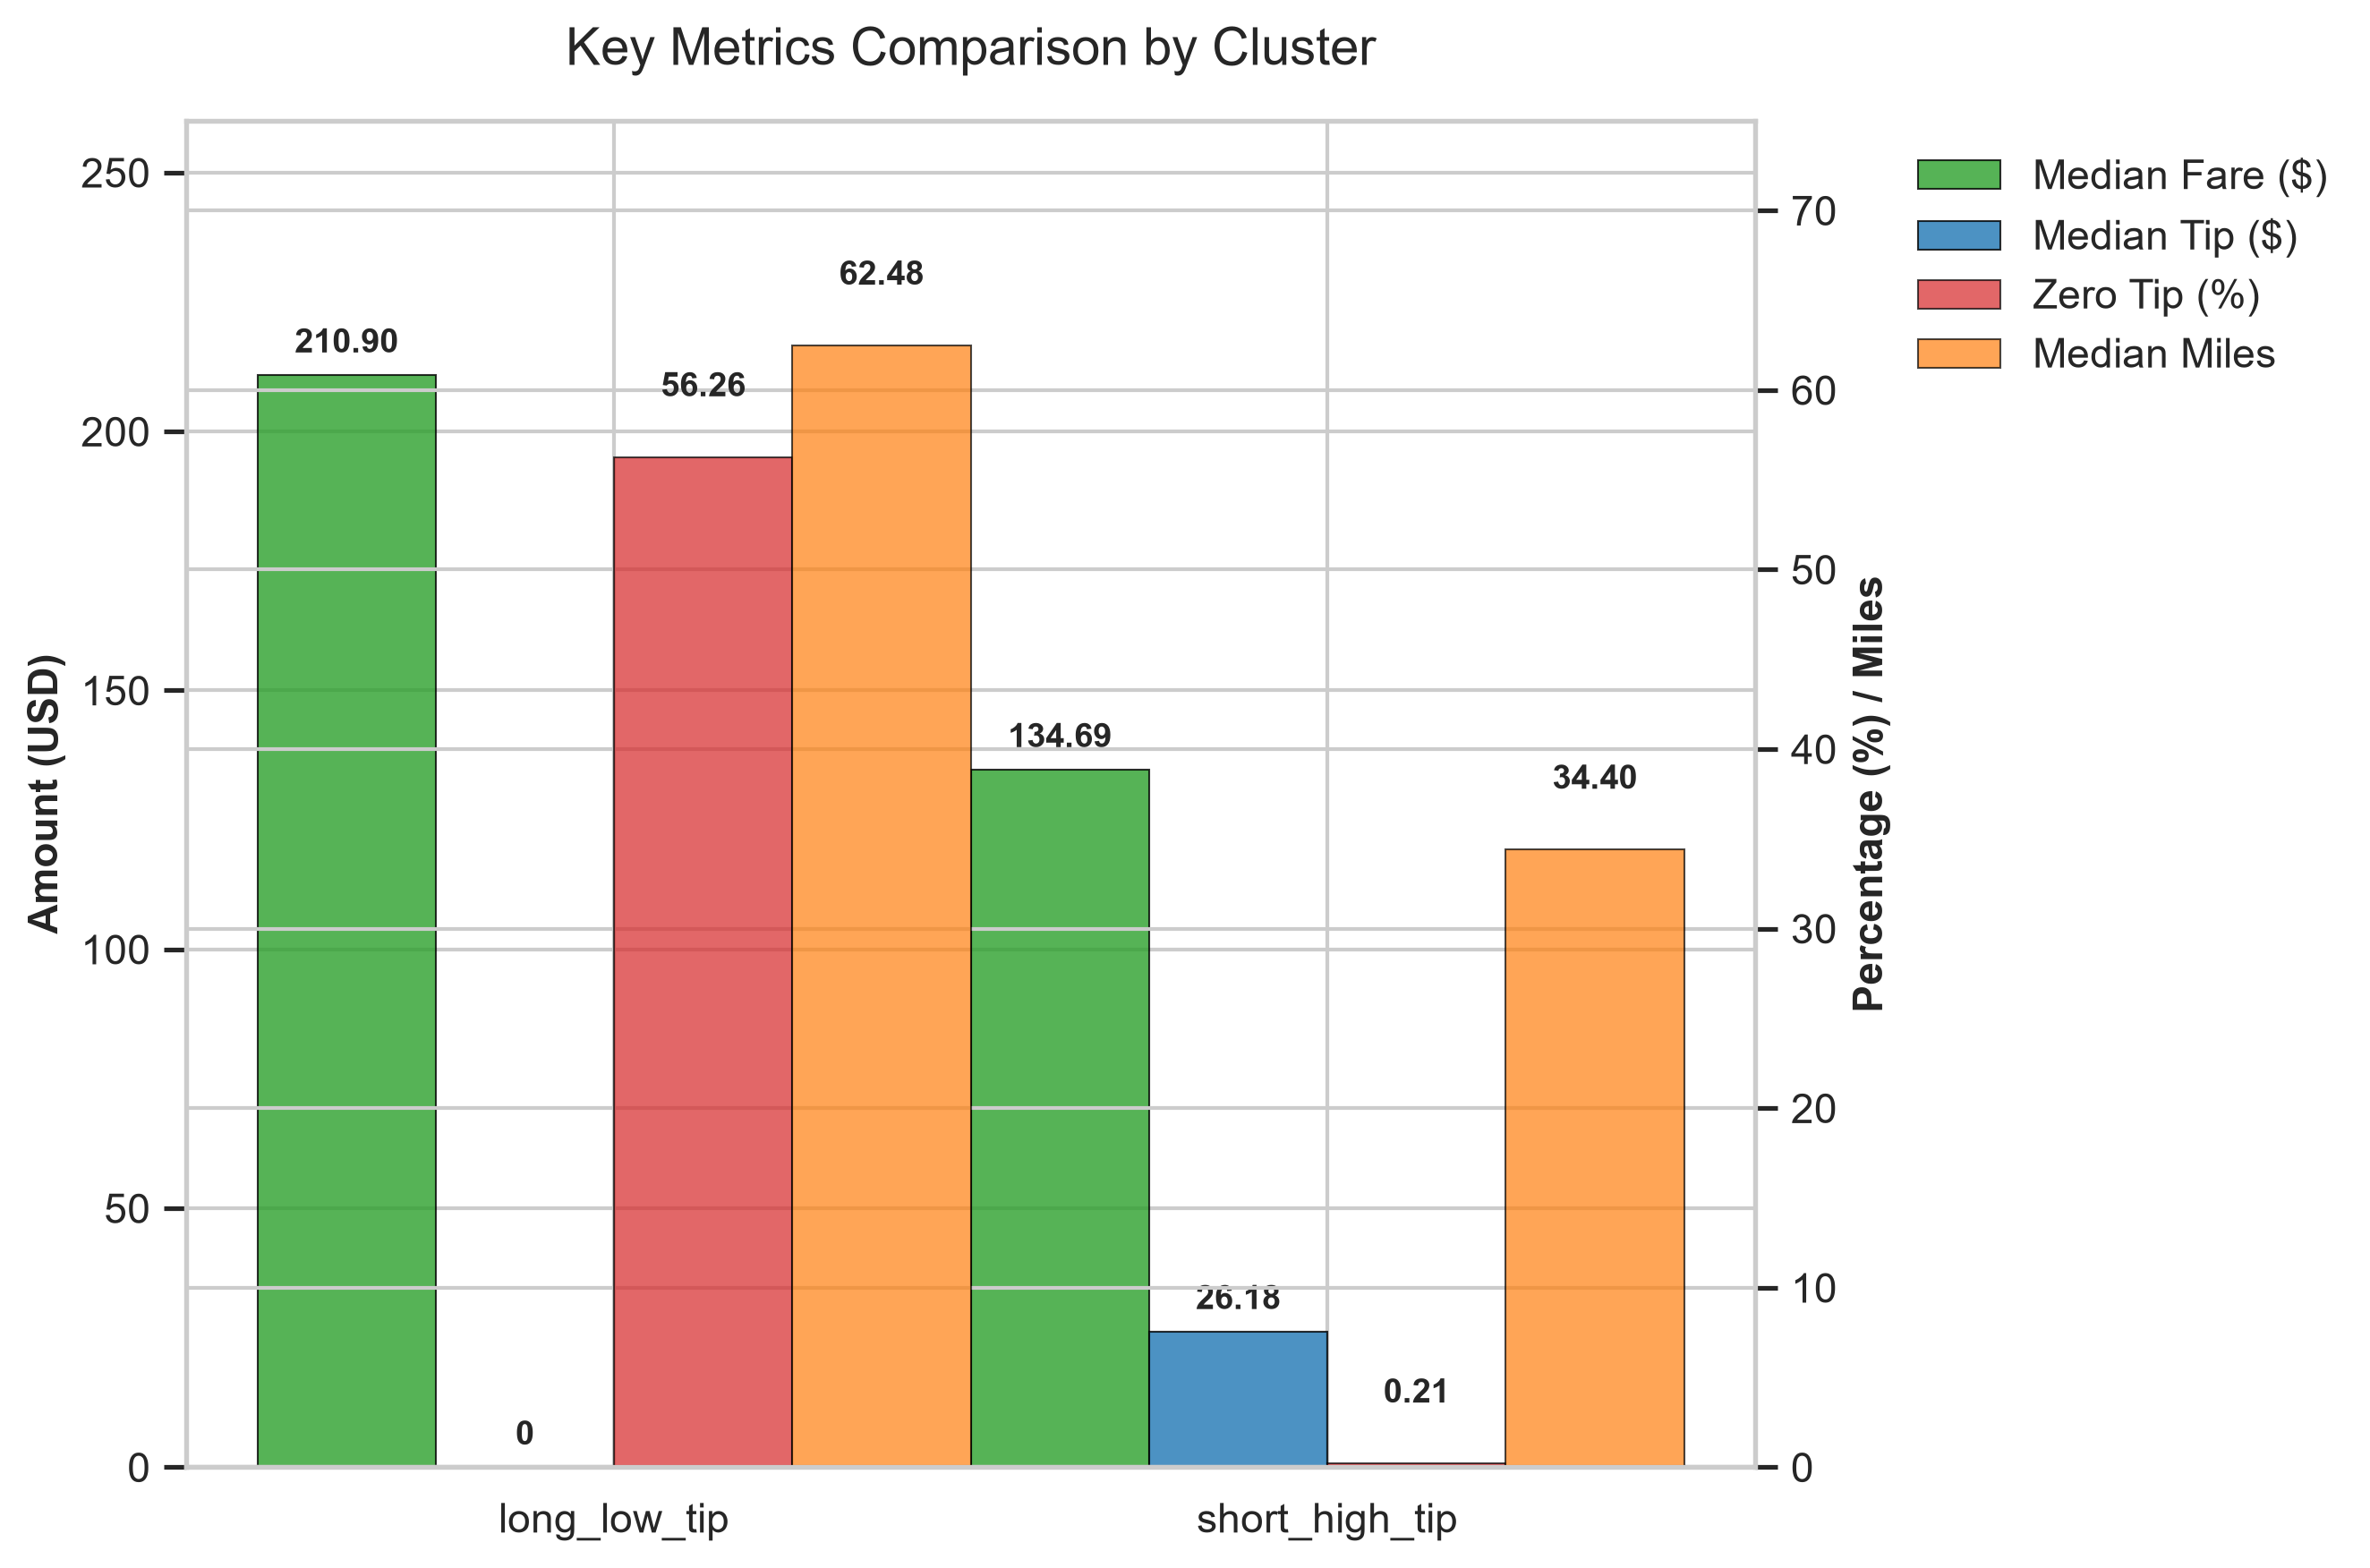
\includegraphics[width=0.80\linewidth]{anomaly_features/viz/1_key_metrics_comparison.png}
\caption{Key metrics by family, in physical units. The comparison is within the flagged set; \emph{long\_low\_tip} is higher on distance, fare and duration, and lower on tip.}
\label{fig:key-metrics}
\end{figure}

\begin{figure}[t]
\centering
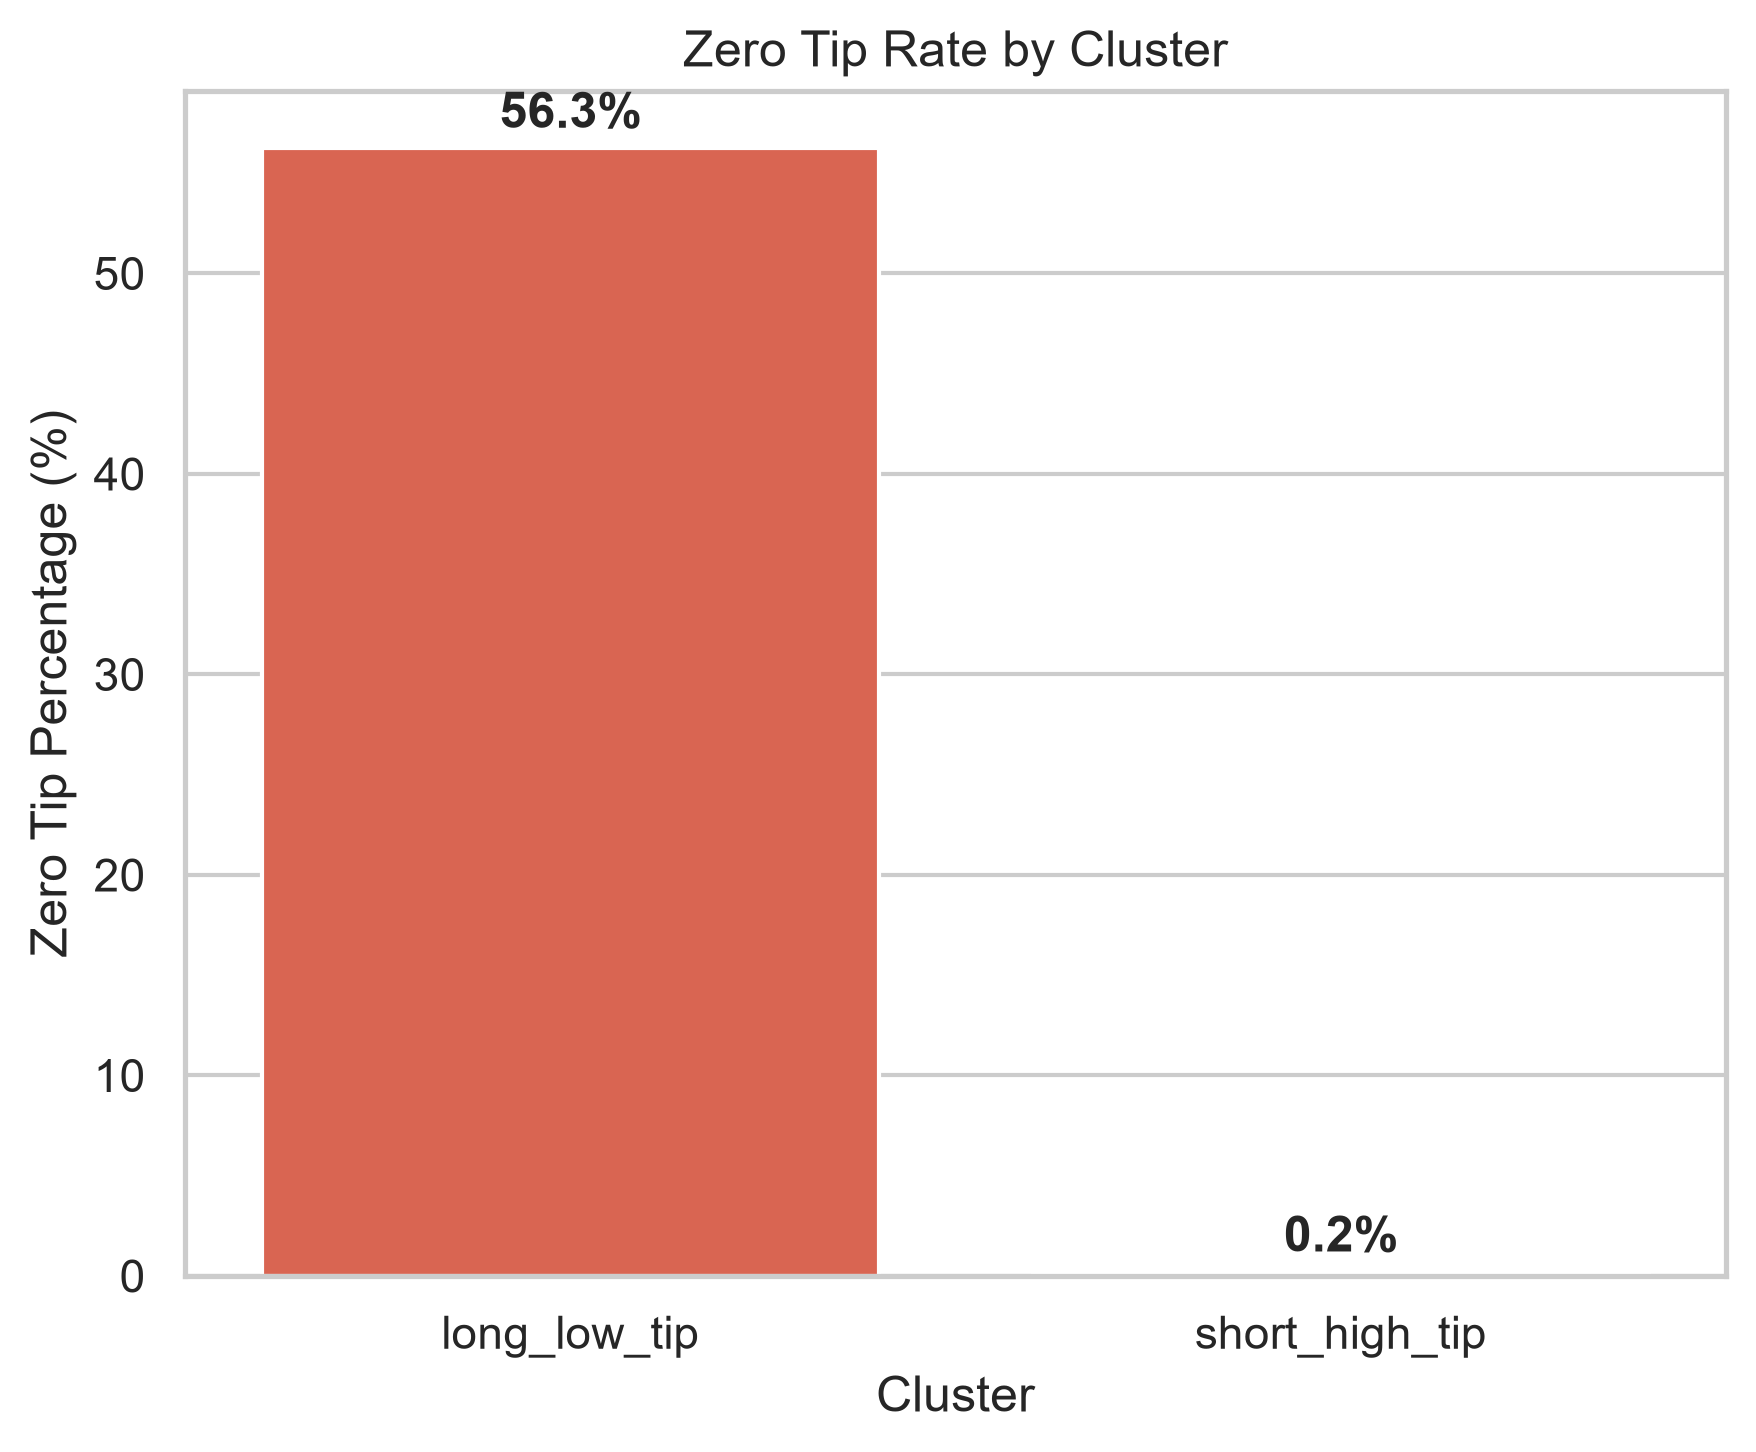
\includegraphics[width=0.55\linewidth]{anomaly_features/viz/4_zero_tip_bar.png}
\caption{Zero-tip share by group: 56.26\% for \emph{long\_low\_tip}, 0.21\% for \emph{short\_high\_tip}, and 15.84\% for the flagged set as a whole. The full population zero-tip share is 80.49\% (document-level measurement).}
\label{fig:zero-tip}
\end{figure}

\subsection{The two families share a mechanism}

Table~\ref{tab:shap} reports the three strongest SHAP drivers for each family, computed on the 2{,}000 highest-scoring flagged trips (1{,}104 \emph{long\_low\_tip} and 896 \emph{short\_high\_tip}); the remaining 11{,}577 flagged trips have no per-row attribution. The top three features are the same, in the same order, for both families, and the per-feature magnitudes differ by only 1.67--3.77\%. The rank correlation between the two profiles is $\rho = 0.9833$.

\begin{table}[t]
\centering
\small
\caption{Top-3 SHAP drivers per family (mean absolute SHAP value). The features are identical and the ordering is identical; only the magnitudes differ.}
\label{tab:shap}
\begin{tabular}{lrrr}
\toprule
Feature & \emph{short\_high\_tip} & \emph{long\_low\_tip} & Relative gap \\
\midrule
\code{log\_tips} & 1.9117 & 1.8410 & 3.77\% \\
\code{speed\_mph} & 1.4674 & 1.4332 & 2.36\% \\
\code{log\_fare} & 1.3364 & 1.3589 & 1.67\% \\
\bottomrule
\end{tabular}
\end{table}

The discrimination test reaches a stronger version of the same conclusion. When the two families are compared on the full attribution profile, the profiles are close enough that the test returns the verdict \emph{indistinguishable}; the two features that do differ are \code{log\_duration} (41.98\% relative gap) and \code{hour\_cos} (43.33\%). We did not train a classifier and report no AUC: with no labels, the discriminability of the two families cannot be tested directly. In other words, the families are separated by the \emph{level} of the same drivers rather than by a different set of drivers. A trip is flagged mainly by its tipping, speed and fare; which family it lands in depends on duration and time of day, not on a different mechanism.

This is a more useful result than a clean separation would have been, because it says that one explanation covers both families. It is also a caution: the SHAP values explain the anomaly score, not the cluster assignment, so Table~\ref{tab:shap} should not be read as a cluster classifier.

\begin{figure}[t]
\centering
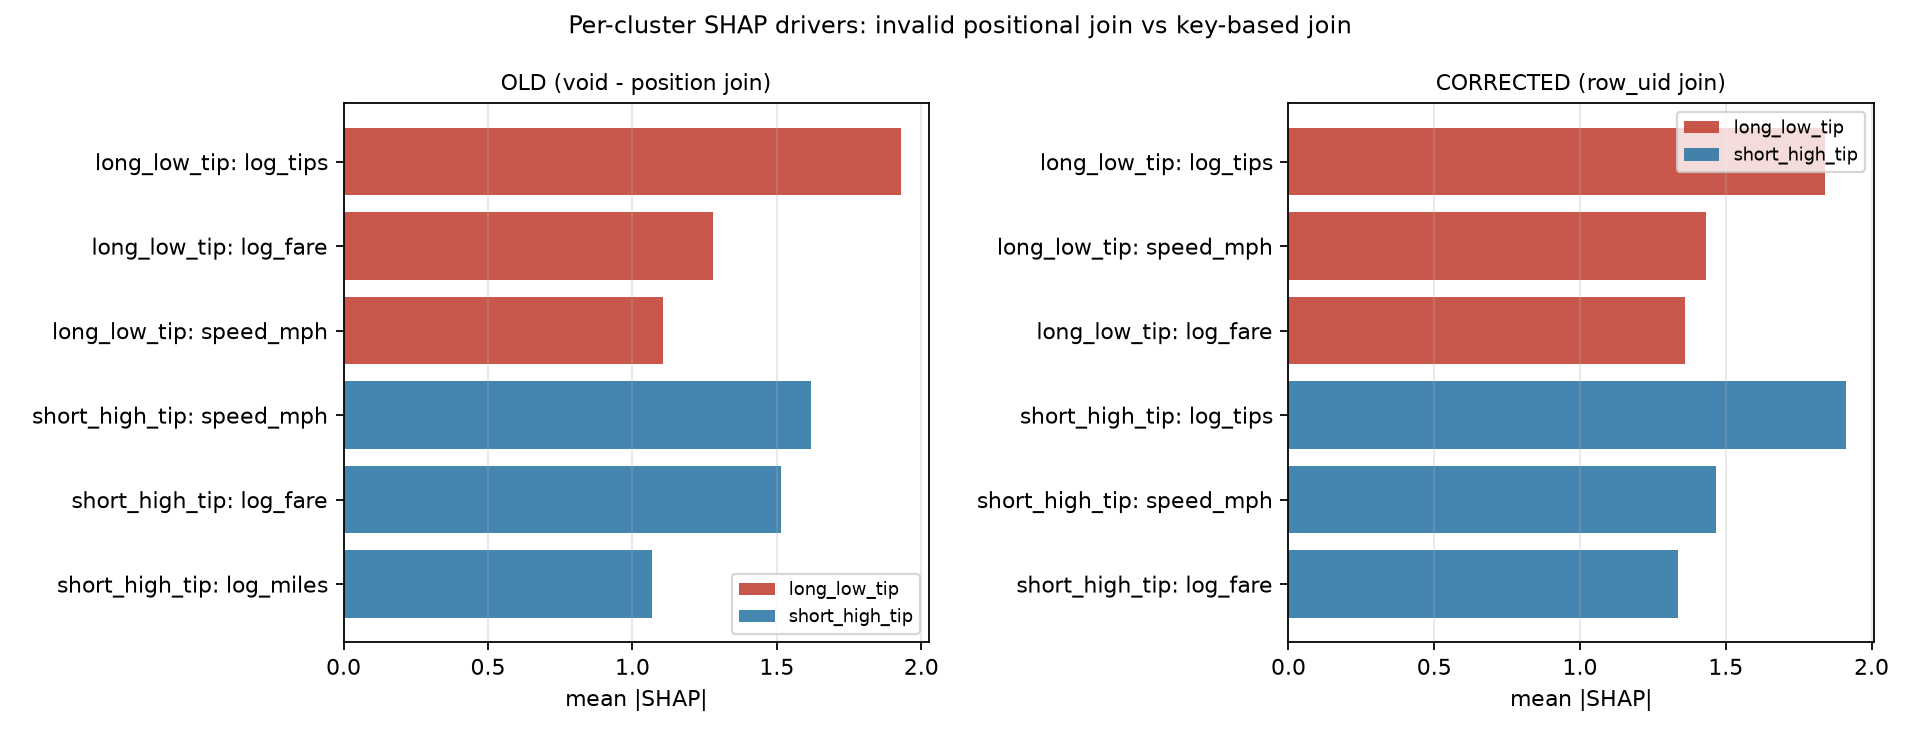
\includegraphics[width=\linewidth]{shap_final/fig_shap_old_vs_corrected.png}
\caption{SHAP attributions before and after the row-alignment fix. The corrected panel is the one used in Table~\ref{tab:shap}; the legacy panel is shown to make the size of the misalignment visible.}
\label{fig:shap-fix}
\end{figure}

\subsection{Parallel scaling}

Table~\ref{tab:scaling} summarises the controlled scaling study. Three results stand out.

\begin{table}[t]
\centering
\small
\caption{Controlled scaling results on 2~M-row (K1, K2) and 1~M-row (S3) subsets. Speed-ups are relative to the two-core configuration or to one thread; intervals are bootstrap 95\% confidence intervals.}
\label{tab:scaling}
\begin{tabular}{llrrr}
\toprule
Experiment & Configuration & Time (s) & Speed-up & 95\% CI \\
\midrule
K1 ($k$-means, $k=2$) & \code{local[2]}, S=30 & 74.86 & 1.00$\times$ & --- \\
 & \code{local[4]}, S=30 & 51.83 & 1.44$\times$ & [1.27, 1.69] \\
 & \code{local[8]}, S=30 & 51.50 & 1.45$\times$ & [1.19, 1.97] \\
K1 ($k$-means, $k=2$) & \code{local[2]}, S=120 & 77.61 & 1.00$\times$ & --- \\
 & \code{local[4]}, S=120 & 47.65 & 1.63$\times$ & [1.47, 1.92] \\
 & \code{local[8]}, S=120 & 50.86 & 1.53$\times$ & [1.37, 1.80] \\
K2 (bisecting, $k=8$) & \code{local[2]}, S=30 & 176.43 & 1.00$\times$ & --- \\
 & \code{local[4]}, S=30 & 144.22 & 1.22$\times$ & [1.09, 1.63] \\
 & \code{local[8]}, S=30 & 98.45 & 1.79$\times$ & [1.23, 2.22] \\
K2 (bisecting, $k=8$) & \code{local[2]}, S=120 & 193.52 & 1.00$\times$ & --- \\
 & \code{local[4]}, S=120 & 189.65 & 1.02$\times$ & [0.99, 1.20] \\
 & \code{local[8]}, S=120 & 102.17 & 1.89$\times$ & [1.85, 2.20] \\
S3 (IF scoring) & 1 thread & 8.51 & 1.00$\times$ & --- \\
 & 4 threads & 2.54 & 3.35$\times$ & [3.32, 3.36] \\
 & 8 threads & 1.94 & 4.38$\times$ & [4.27, 4.44] \\
 & 20 threads (\code{-1}) & 2.12 & 4.01$\times$ & [3.82, 4.19] \\
\bottomrule
\end{tabular}
\end{table}

First, more cores are not uniformly better. The two-cluster $k$-means gains 1.44--1.63$\times$ up to four cores and gains nothing at eight; at the larger shuffle setting, eight cores are about 6.7\% slower than four. We report this as ``no evidence that eight beats four'', not as equality, because we did not compute an interval for the 4-vs-8 difference; with four runs per cell and overlapping intervals that comparison is not supported.

Second, the bisecting $k$-means at $k=8$ does benefit from eight cores, reaching 1.79--1.89$\times$ over two cores, with a pooled estimate of 1.77$\times$ when the post-hoc replication is combined with the primary runs. The pooled figure is post-hoc (four primary and four replication runs, $n=8$), unbalanced (only this cell has eight runs), has no same-day baseline, and includes a replication median 10.1\% slower than the primary cell; the pooled median is 99.61~s against 98.45~s. The difference from K1 is consistent with the structure of the algorithm: bisecting $k$-means performs more, smaller fits, so the per-fit serial fraction is lower and additional cores find work to do.

Third, thread-level parallelism in the forest scales further than the Spark-level jobs, because there is no shuffle and no task-launch overhead: scoring 1~M rows with eight threads is 4.38$\times$ faster than with one, and using all 20 logical cores is \emph{slower} than eight (4.01$\times$), which is the signature of oversubscription.

Amdahl's model fits the Spark experiments with a serial fraction of $\alpha = 0.295$--$0.375$. That number is the honest summary of this section: roughly a third of each Spark job's runtime does not benefit from extra cores, which caps the achievable speed-up at about 3$\times$ regardless of how many cores are added.

\begin{figure}[t]
\centering
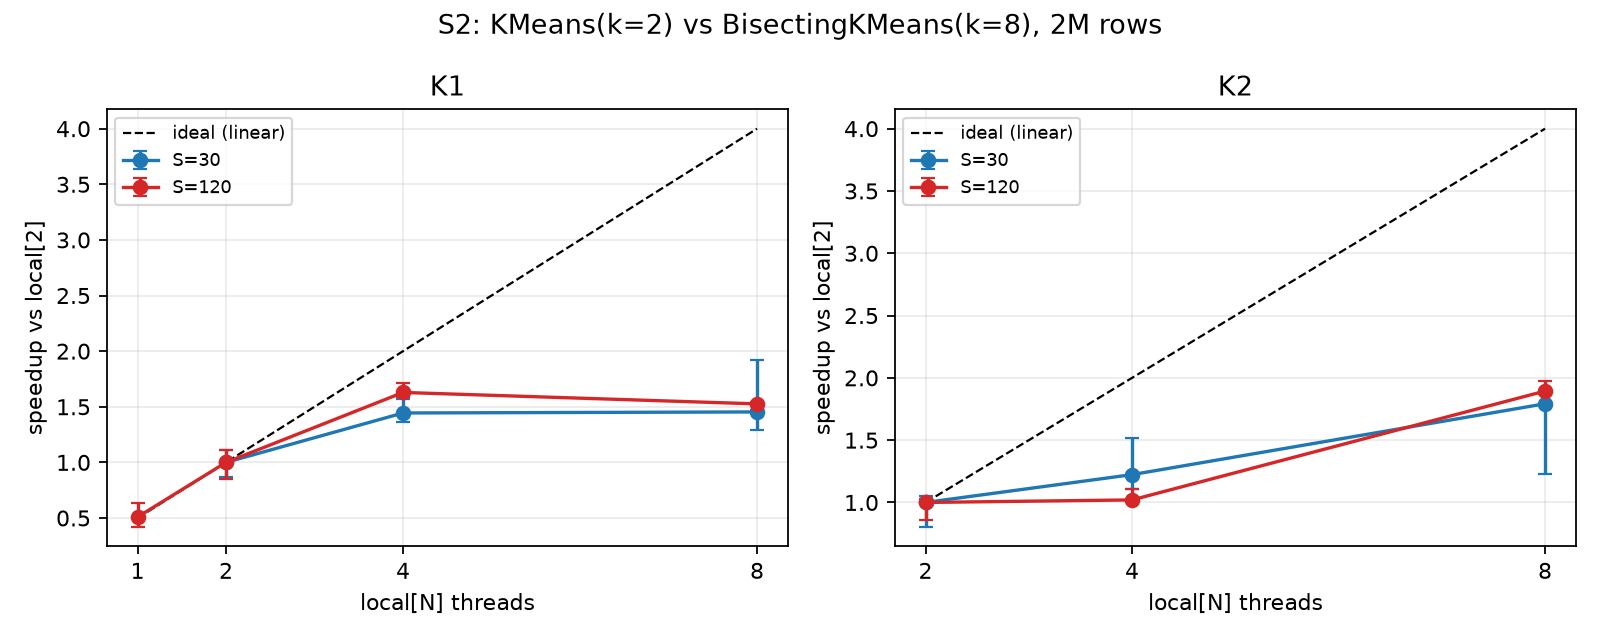
\includegraphics[width=0.82\linewidth]{scaling_study/figures/s2_speedup.png}
\caption{Measured speed-up for the two Spark clustering experiments (K1, K2) as cores increase, with bootstrap intervals. The dashed line is linear speed-up.}
\label{fig:s2-speedup}
\end{figure}

\begin{figure}[t]
\centering
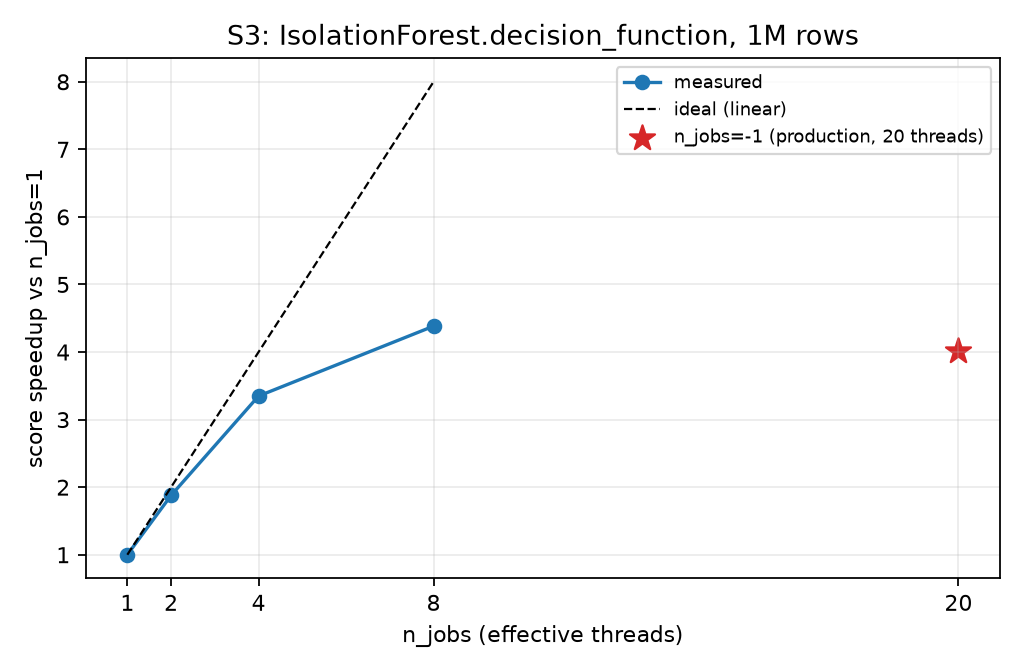
\includegraphics[width=0.78\linewidth]{scaling_study/figures/s3_speedup.png}
\caption{Thread-level speed-up for Isolation Forest scoring on 1~M rows. Beyond eight threads the curve turns down, which is the cost of oversubscription rather than a measurement artefact.}
\label{fig:s3-speedup}
\end{figure}

A final number belongs in this section but not in the table. The largest single fit we ran was a bisecting $k$-means with $k=8$ over the full 46.7~M-row first-stage sample, which completed in 2{,}198~s on \code{local[*]}. It is a feasibility datum, not a scaling result: $K=8$ was later rejected, the production model is a single $k$-means with $k=2$, and the run exists because we needed to know whether such a fit was possible on this machine at all.

% ---------------------------------------------------------------------
\part{Business Intelligence}

\section{Descriptive Findings}
\label{sec:bi}

All results in this part are computed from the cleaned table described in
Section~\ref{sec:data}. Three populations are in play, and every number below
names the one it is taken from:

\begin{itemize}
\item $N_{\text{all}} = 471{,}960{,}468$ --- every record in the release;
\item $N_{\text{wait}} = 467{,}359{,}108$ --- records with
      \code{wait\_valid = 1}, that is a request-to-pickup wait between 0 and
      120~minutes as defined in Section~\ref{sec:data}. The bound removes
      missing, negative \emph{and} implausibly long waits;
\item $N_{\text{flag}} = 467{,}142{,}106$ --- records
      passing all three validation flags. Because \code{wait\_valid} is one of
      the three, the fully validated set is a subset of the wait-valid set and
      contains 217{,}002 fewer rows.
\end{itemize}

Trip volume and share are computed over $N_{\text{all}}$, and every
waiting-time statistic over $N_{\text{wait}}$. $N_{\text{flag}}$ is used only by
the unsupervised track in Part~I, where all three flags must hold before
sampling. Weekly patterns and longer waits in specific periods provide a basis
for testing service improvements.

% ---------------------------------------------------------------------
\subsection{Trip patterns across time and location}

This part never reads trip-level rows. The 471.96~million records are
aggregated into two derived tables, both written as Parquet partitioned by
pickup date: a detailed table \code{l1\_detail} with 8{,}651{,}895 rows at
day~$\times$~pickup-zone~$\times$~hour~$\times$~platform granularity, and an
overview table \code{l2\_overview} with 4{,}421{,}839 rows at
day~$\times$~borough~$\times$~hour. Together they occupy 558~MB in 1{,}462
files across 731 daily partitions, against 11.6~GB for the trip-level Parquet
they are built from. Every chart in this part reads one of these two
aggregates, which is why the analysis runs on a few hundred megabytes instead
of 4.7 hundred million rows.

Two conventions hold throughout. Platform is a licensee code:
\code{HV0003} is reported as Uber and \code{HV0005} as Lyft, which is a
licensee-level mapping and not a brand-level one. And each chart states the
population it uses: volume charts are computed over $N_{\text{all}}$ and
waiting-time charts over $N_{\text{wait}}$.

\subsubsection{Weekly variation in daily trips}

\begin{figure}[t]
\centering
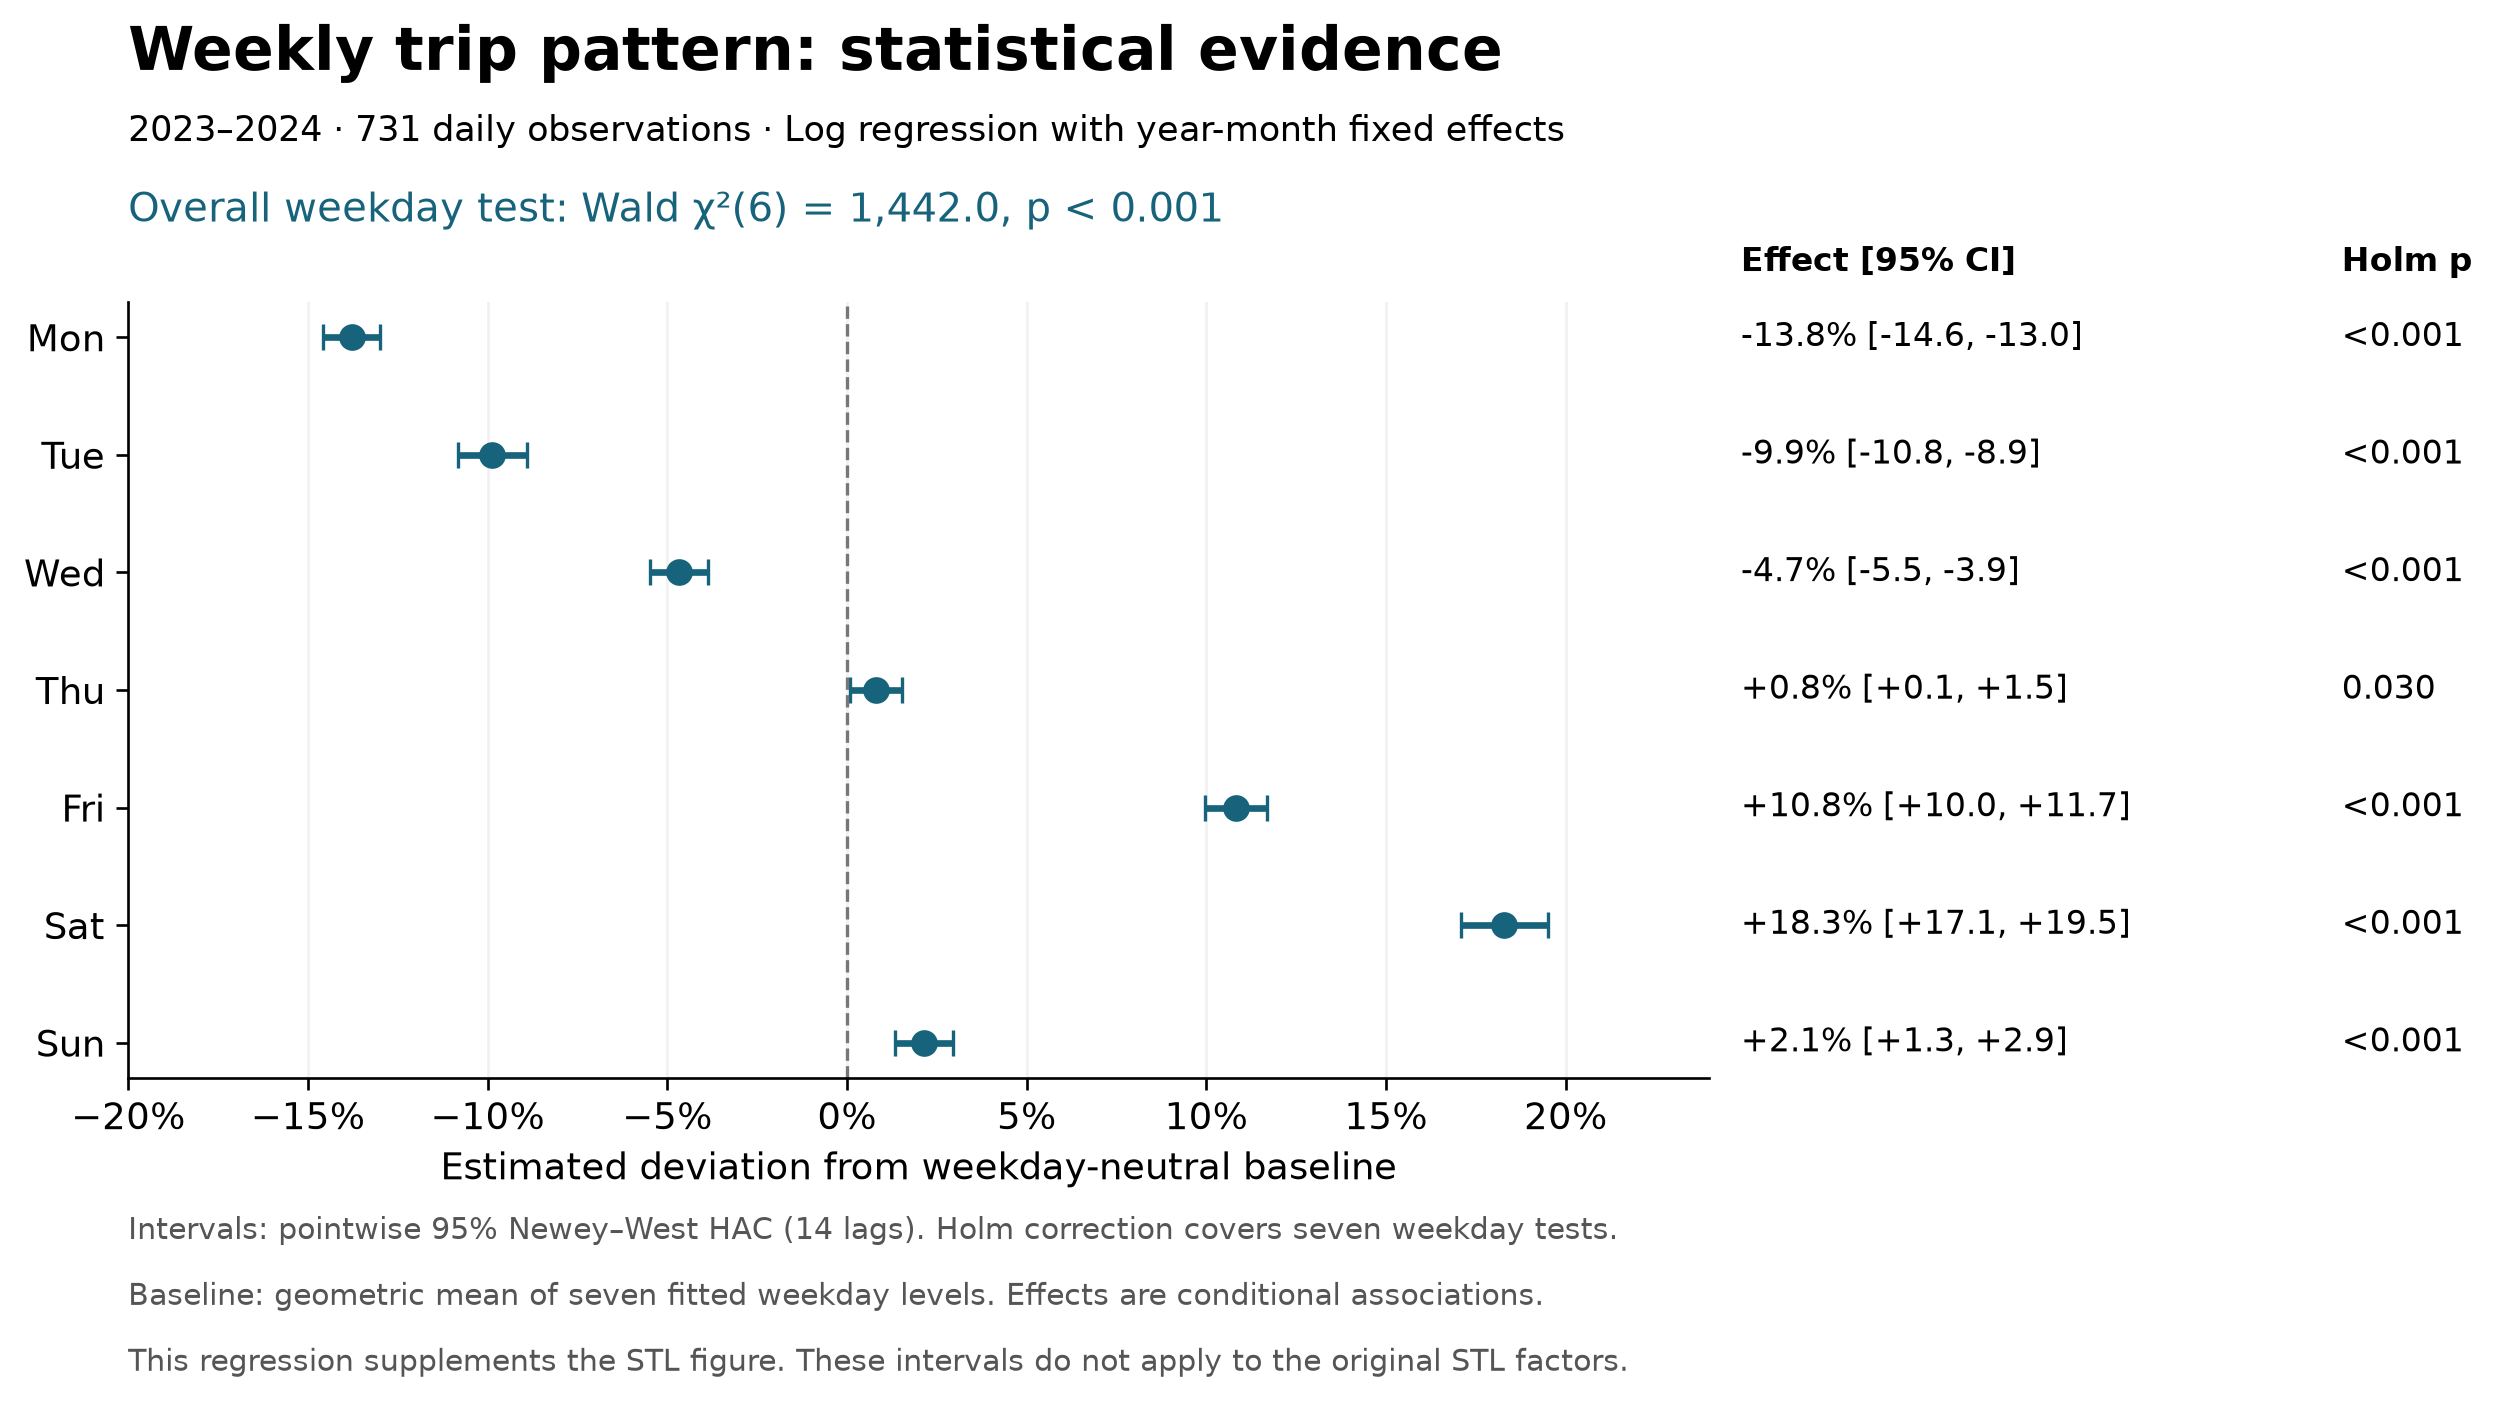
\includegraphics[width=0.82\linewidth]{bi/fig01_weekday_effect.png}
\caption{Estimated weekday differences in daily trip volume
($N_{\text{all}}$), with pointwise 95\% HAC confidence intervals.}
\label{fig:bi-weekday}
\end{figure}

The regression of log daily trips used all recorded trips ($N_{\text{all}}$)
across 731 days, weekday indicators and year-month fixed effects for the
24 calendar months. Because consecutive days
share weather, holidays and residual demand, the standard errors are
heteroskedasticity- and autocorrelation-consistent (HAC, Newey--West) with
14 lags rather than the ordinary OLS ones, and the intervals in
Figure~\ref{fig:bi-weekday} are pointwise 95\% intervals on that basis. The
joint test on the six weekday indicators gives $\chi^2(6) = 1{,}442.0$ with
$p < 0.001$.

Saturday had the highest adjusted trip level, followed by Friday, while Monday
had the lowest. The percentages are relative to the geometric mean of the seven
fitted weekday levels, which is the natural baseline in a log-linear model with
weekday dummies: it is the level of an average week, not the level of any one
day. On that baseline Saturday was 18.30\% higher, Friday was 10.83\% higher
and Monday was 13.78\% lower. Related forecasting work uses spatial and temporal
information to predict short-term ride-service demand~\cite{ke2017}; the
weekday effect sizes reported here are estimated from our NYC data.

\subsubsection{Monthly variation and annual growth}

\begin{figure}[t]
\centering
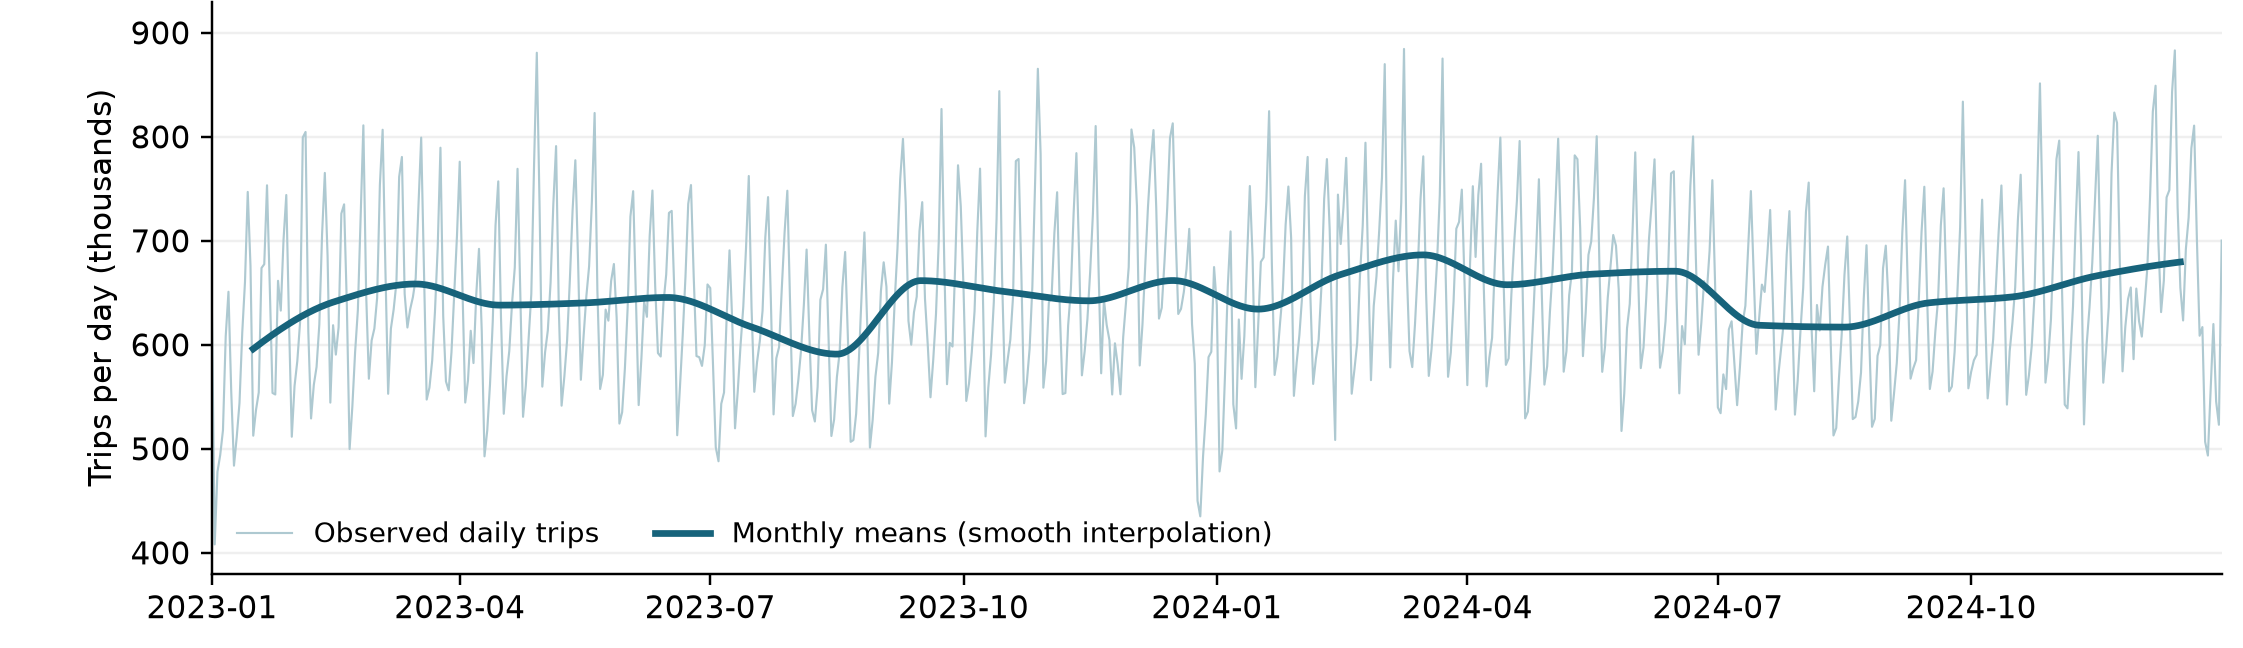
\includegraphics[width=\linewidth]{bi/fig02_monthly_trend.png}
\caption{Observed daily trips and a smooth curve through monthly daily averages
($N_{\text{all}}$).}
\label{fig:bi-monthly}
\end{figure}

Total trips rose from 232{,}490{,}020 in 2023 to 239{,}470{,}448 in 2024,
an increase of 3.00\% (counts over $N_{\text{all}}$). The average per day rose
by 2.72\%, after accounting for 366 days in 2024 and 365 in 2023:
\[
\left(\frac{239{,}470{,}448}{232{,}490{,}020}
\times\frac{365}{366}-1\right)\times100\% \approx 2.72\%.
\]
July and August were relatively quiet in both years, with August recording the
lowest monthly daily average.
Two years of data cannot establish a stable annual seasonal pattern
(Figure~\ref{fig:bi-monthly}).

\subsubsection{Geographic distribution}

\begin{figure}[t]
\centering
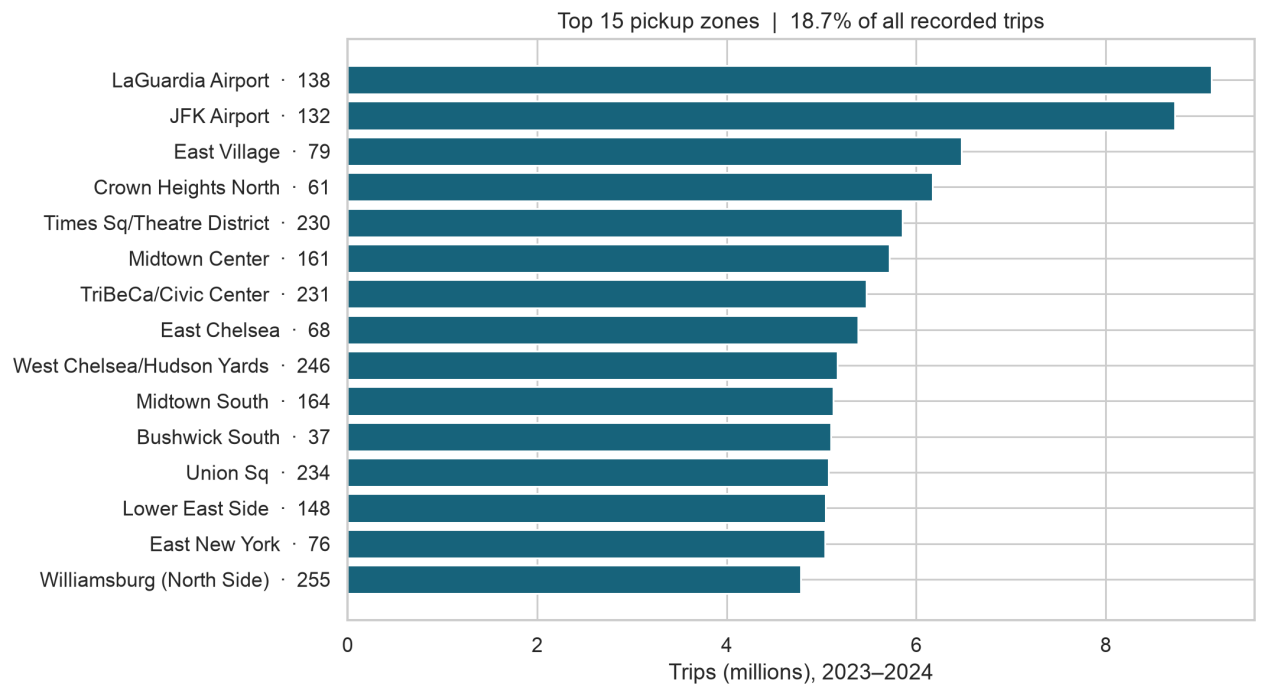
\includegraphics[width=0.82\linewidth]{bi/fig03_top15_zones.png}
\caption{Top 15 pickup zones by trip count, 2023--2024. The 15 zones account
for 18.7\% of the 472.0~million recorded trips ($N_{\text{all}}$).}
\label{fig:bi-zones}
\end{figure}

The 15 busiest pickup zones account for 18.7\% of all recorded trips
($N_{\text{all}}$). LaGuardia Airport and JFK Airport rank first and second.
Several central Manhattan and Brooklyn zones also appear near the top. The
remaining 81.3\% of trips are picked up outside these 15 zones, so planning
should consider both major pickup locations and the wider service area
(Figure~\ref{fig:bi-zones}).

\subsubsection{Trip volume by weekday and hour}

\begin{figure}[t]
\centering
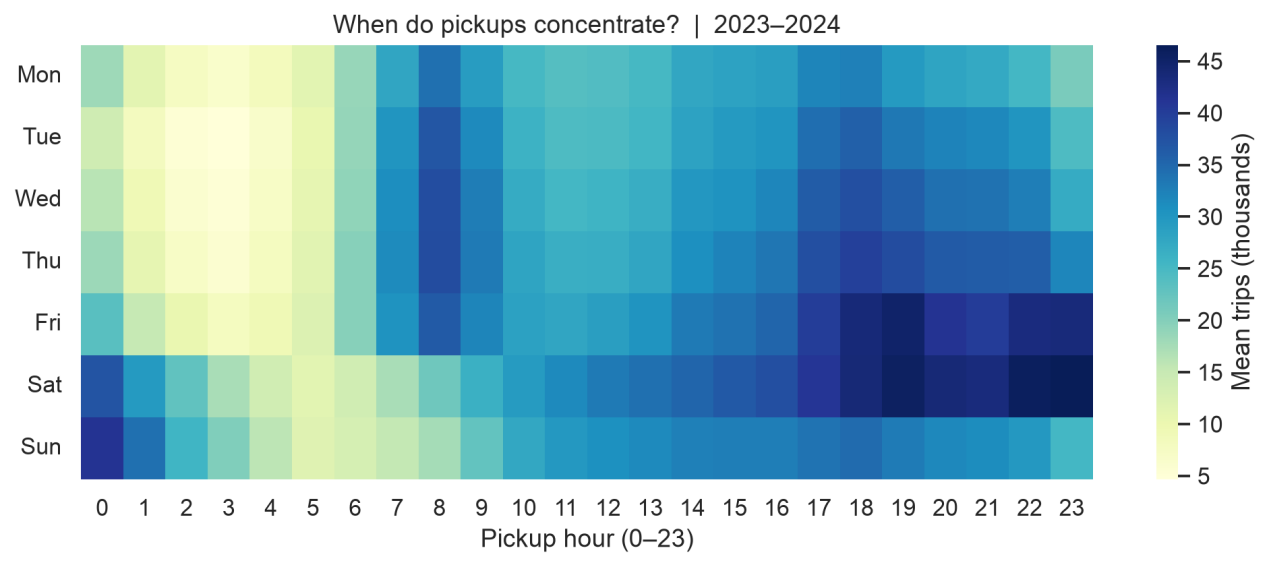
\includegraphics[width=0.92\linewidth]{bi/fig04_weekday_hour_heat.png}
\caption{Average trips by weekday and pickup hour, in thousands
($N_{\text{all}}$).}
\label{fig:bi-weekday-hour}
\end{figure}

Weekday mornings show a local peak around 08:00, followed by another busy period
from 17:00 to 19:59. High volumes continue into the late evening on Fridays and
Saturdays, particularly from 18:00 to 23:59. Saturday from 23:00 to 23:59 is the
busiest weekday-hour combination, averaging about 46{,}500 recorded trips per
Saturday during that hour, using $N_{\text{all}}$
(Figure~\ref{fig:bi-weekday-hour}).

\subsubsection{Waiting time by weekday and hour}

\begin{figure}[t]
\centering
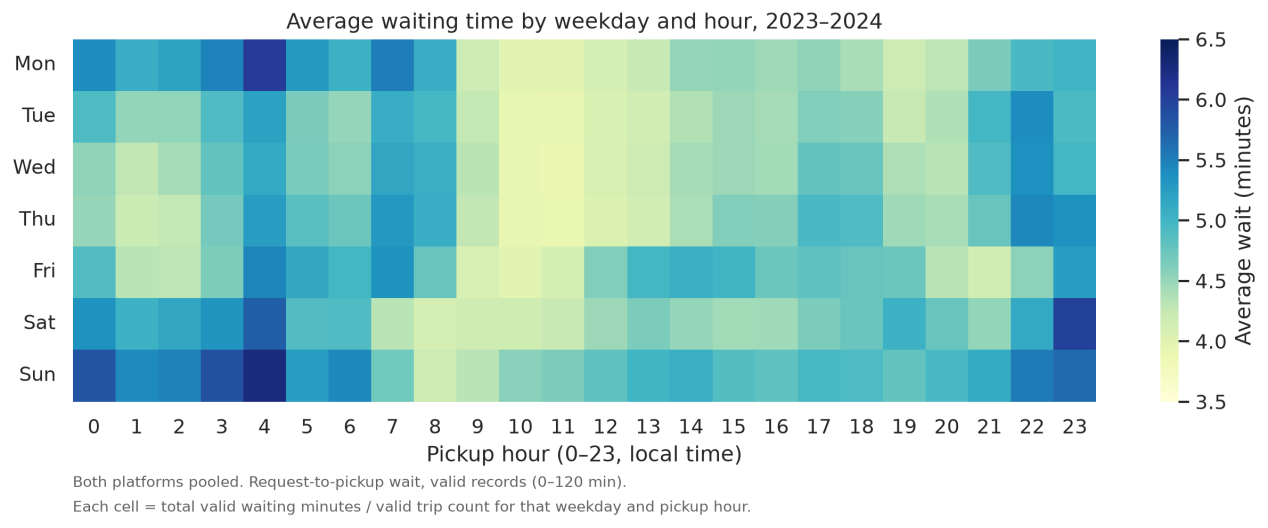
\includegraphics[width=0.92\linewidth]{bi/fig05_wait_weekday_hour.png}
\caption{Average request-to-pickup waiting time by weekday and pickup hour,
restricted to \code{wait\_valid = 1}.}
\label{fig:bi-wait-hour}
\end{figure}

Waiting times are generally longer during the early morning, particularly from
00:00 to 04:59 on Saturdays, Sundays and Mondays. They are also elevated at
23:00 on Saturdays and Sundays. Weekday waits are usually shorter around 10:00
to 11:59. The longest average is 6.26~minutes on Sundays from 04:00 to 04:59
(Figure~\ref{fig:bi-wait-hour}).

All waiting-time figures in this part are computed over $N_{\text{wait}}$, that
is, waits between 0 and 120~minutes. The bound is not neutral: it removes
missing and negative records, but it also cuts the genuinely long tail, and the
share removed is not constant across hours, boroughs or platforms. A period
whose waits are trimmed more heavily will therefore look faster than it is, so
every waiting-time comparison below should be read with that in mind. Waiting
time in a competitive market reflects search frictions as well as demand,
which is why the two are treated as separate questions
here~\cite{frechette2019}.

\subsubsection{Business insights for service planning}

The four points below are hypotheses that the descriptive results make worth
testing, not recommendations. Each would need its own cost and volume case
before anything is changed, and Section~\ref{sec:discussion} explains why.

\begin{itemize}
\item \emph{Driver availability should follow the weekly pattern.} Friday and
      Saturday evenings are the strongest candidates for additional coverage;
      local trip counts should decide which zones, including the airports and
      the busy central areas.
\item \emph{Waiting time is worth assessing separately from trip volume.} Some
      early-morning periods have relatively few trips but long waits, which is
      where a targeted incentive would be easiest to evaluate.
\item \emph{The intersection of high volume and long waits is the first place
      to look.} Late Saturday evening satisfies both conditions.
\item \emph{Capacity could be adjusted gradually in quieter months.} July and
      August were quieter in both observed years, but two years cannot
      distinguish a seasonal pattern from a temporary one.
\end{itemize}

% ---------------------------------------------------------------------
\subsection{Uber and Lyft comparison}

\subsubsection{Trip share and regional mix}

\begin{figure}[t]
\centering
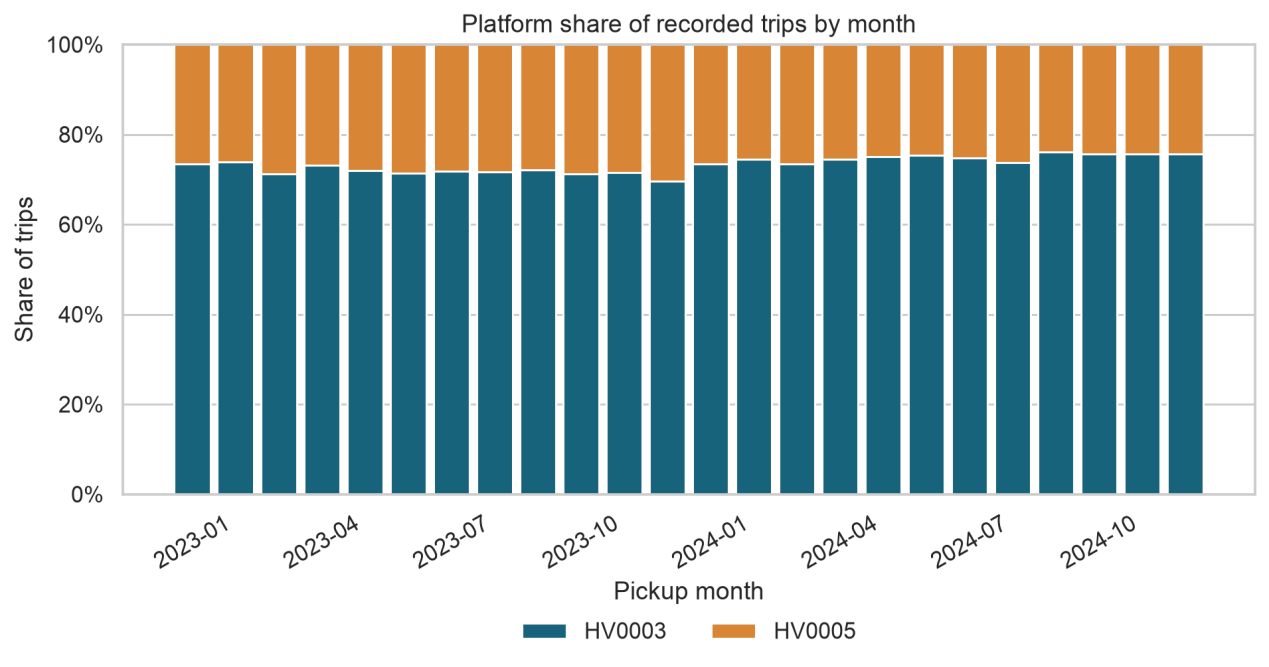
\includegraphics[width=0.80\linewidth]{bi/fig06_platform_share.png}
\caption{Monthly trip shares within the combined Uber and Lyft dataset
($N_{\text{all}}$).}
\label{fig:bi-share}
\end{figure}

\begin{figure}[t]
\centering
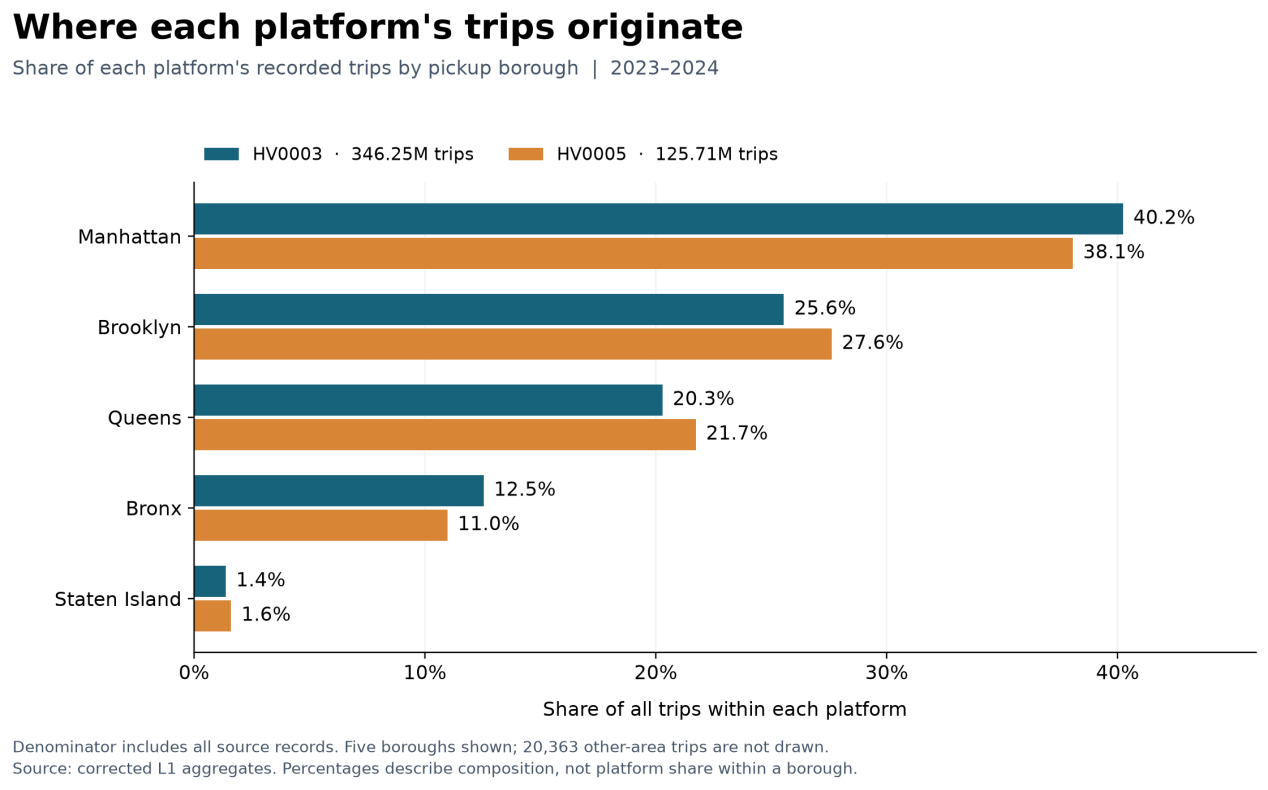
\includegraphics[width=0.72\linewidth]{bi/fig07_borough_mix.png}
\caption{Distribution of each platform's trips by pickup borough
($N_{\text{all}}$).}
\label{fig:bi-borough}
\end{figure}

The two platforms rank the pickup boroughs almost identically, with Manhattan
first, followed by Brooklyn and Queens (Figure~\ref{fig:bi-borough}). The
monthly share of Uber rises from 73.5\% in January 2023 to
75.6\% in December 2024, within a range of 69.6--76.1\%, while Lyft falls by
about 2.1 percentage points over the same window
(Figure~\ref{fig:bi-share}). The movement is gradual but directional. In a
separate comparison of Uber and taxis, Cramer and Krueger report higher
capacity utilisation for Uber drivers~\cite{cramer2016}.

\subsubsection{Waiting time across the day}

\begin{figure}[htbp]
\centering
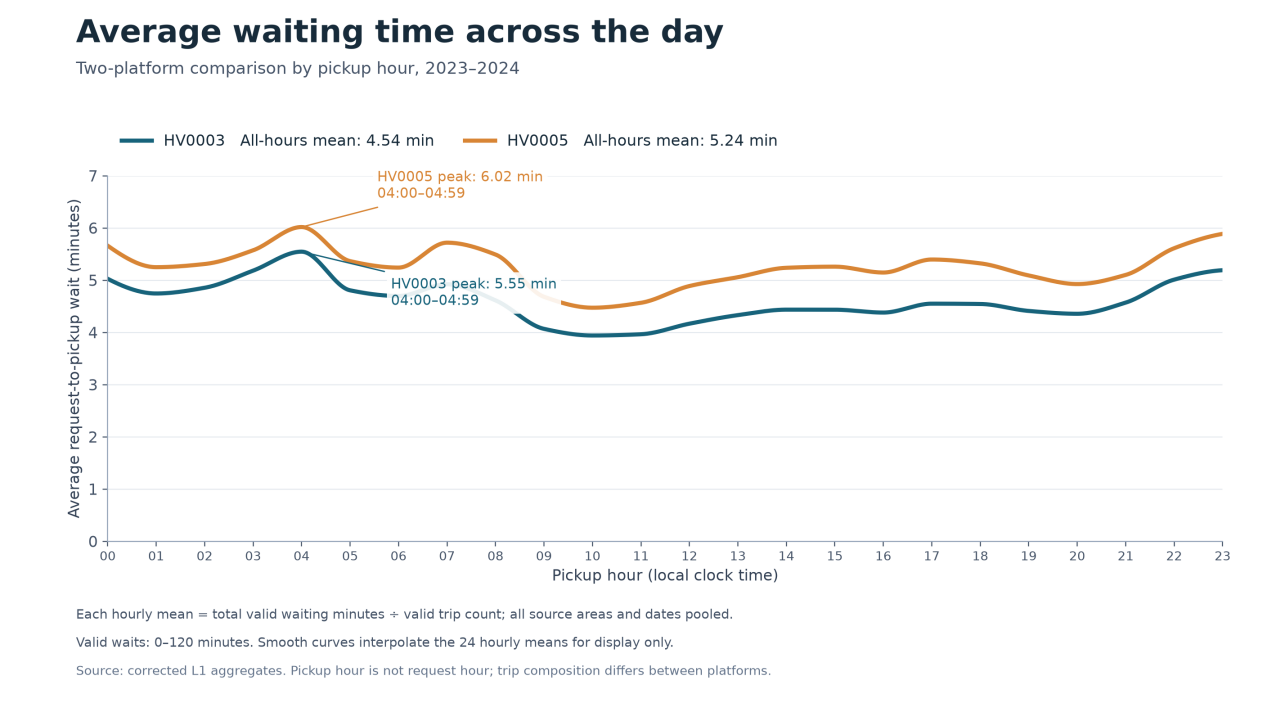
\includegraphics[width=0.86\linewidth]{bi/fig08_wait_by_platform.png}
\caption{Average request-to-pickup waiting time by platform and pickup hour,
restricted to \code{wait\_valid = 1}.}
\label{fig:bi-wait-platform}
\end{figure}

Lyft has higher average waits in all 24 hourly groups: 5.24~minutes overall,
compared with Uber's 4.54~minutes, a gap of about 42~seconds
(Figure~\ref{fig:bi-wait-platform}). Both overall figures are weighted by trip
count over all hours and days, so they describe the average trip rather than
the average hour. A gap of 42~seconds is small against the trimming sensitivity
described above, so it is evidence of a consistent direction rather than of a
precisely estimated magnitude.

\subsubsection{Potential areas for Lyft service pilots}

\begin{figure}[htbp]
\centering
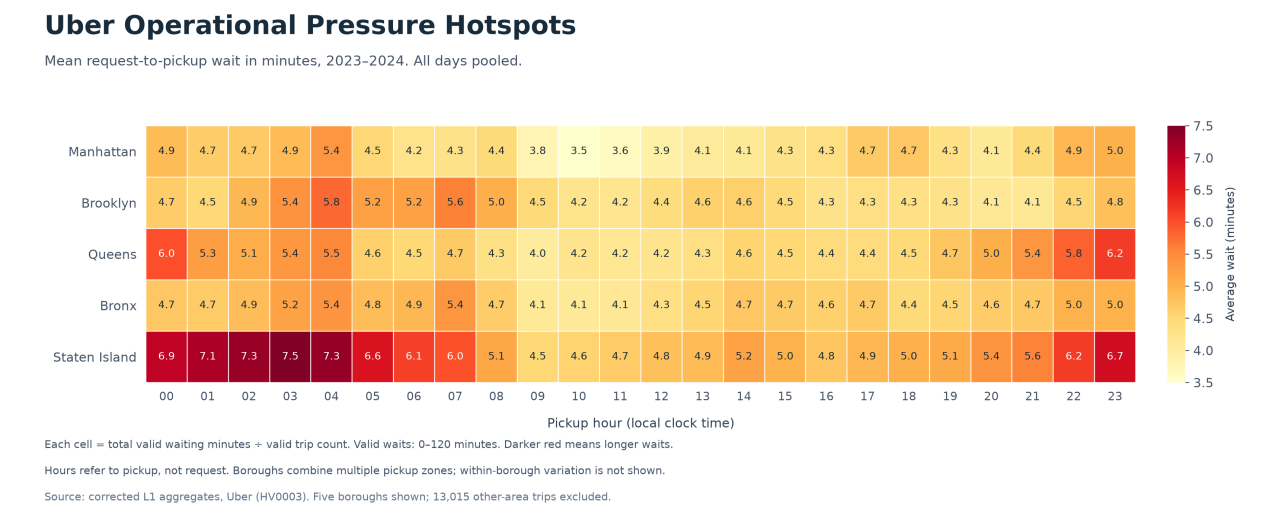
\includegraphics[width=0.86\linewidth]{bi/fig09_uber_pressure.png}
\caption{Uber waiting-time hotspots by pickup borough and pickup hour,
2023--2024. The quantity the chart labels operational pressure is the mean
request-to-pickup wait in minutes: each cell is total valid waiting minutes
divided by valid trip count, over $N_{\text{wait}}$.}
\label{fig:bi-pressure}
\end{figure}

The highest mean wait is 7.49~minutes in Staten Island from 03:00 to 03:59;
Queens reaches 6.17~minutes from 23:00 to 23:59
(Figure~\ref{fig:bi-pressure}). Both are
borough-hour cells, not borough averages. The Staten Island cells rest on far
fewer trips than the Manhattan ones, so they locate candidates for a pilot;
they do not estimate the typical wait in a borough. Waiting time and spatial
access are jointly determined in this market, which is why a single cell is
read as a location to investigate rather than as a
result~\cite{buchholz2022}.

\subsubsection{Business insights for Lyft}

\begin{itemize}
\item \emph{Candidate cells, not boroughs.} The early-morning Staten Island cells
      and the late-night Queens cells are where Uber's waits are longest, so
      they are the first places to check. Whether Lyft has enough volume and
      share there is a separate question, and a long Uber wait is not by itself
      an opportunity for Lyft.
\item \emph{A pilot is worth testing between 23:00 and 04:59.} It should start
      in cells that have both meaningful trip volume and long waits, and it
      should be judged on whether the shorter waits justify the incentive cost.
\item \emph{Evaluate before expanding.} Compare waits and completed trips with
      comparable untreated cells, and include incentive costs and cancellations
      where those data exist.
\end{itemize}

\part{Synthesis}

\section{Discussion}
\label{sec:discussion}

\subsection{Two tracks, two resolutions}

Part~I and Part~II look at the same 471.96~M trips at different resolutions. The BI component describes the population: how demand and waiting time are distributed across hour, zone and platform, and which validity filter each statement needs. The unsupervised component isolates 13{,}577 rows and explains why each was flagged. Neither track has a ground-truth label, and neither can substitute for the other: a population average says nothing about an individual extreme trip, and a flag says nothing about how common its pattern is.

One contrast makes the relationship concrete. The modal outcome of the BI layer is a short, cheap, untipped trip: 80.49\% of all trips carry no tip. Only 15.84\% of the flagged trips do, because flagging selects for long, expensive rides rather than for the zero-tip mass, and within the flagged set the zero-tip share is concentrated in one family (56.3\%). Anomaly and normality are therefore not opposites in this data. The flagged rows are unusual in ways the population distribution can measure but cannot explain, which is exactly why both tracks belong in the same report.

\subsection{Three defects worth reporting}
\label{sec:bugs}

The most transferable part of this project is not the cluster profile but the three defects we found in our own pipeline. Each was silent, each produced a number that looked publishable, and each was caught only by an independent check.

\textbf{A positional join.} The first SHAP analysis joined the flagged trips to the attribution matrix by row order. The two jobs did not return the same number of rows, and the legacy script truncated the longer side to 2{,}000 rows; the only trace was a log line reading \emph{``Row count mismatch. Truncating clustered data to 2000 rows.''} Because both tables were sorted differently, the attributions were attached to the wrong trips. The fix was to assign \code{row\_uid} with \code{monotonically\_increasing\_id()} before any join and to join on it. After the fix, all 13{,}577 rows match the cluster table and the largest difference in the joined features is $7.1 \times 10^{-15}$; attributions exist for the 2{,}000 highest-scoring trips analysed in Section~\ref{sec:results}, not for all 13{,}577.

\textbf{A unit error of a factor of 60.} Duration was treated as hours in the consistency features while the rest of the pipeline used minutes. The error is invisible in descriptive statistics because every derived speed is scaled by the same factor, so the distribution still looks plausible. We caught it by testing the algebraic identity that must hold if the units are right: with minutes, the residual median is 0.0 and the maximum over 2~M rows is $8.9 \times 10^{-16}$; with hours, the residual median is 2.60 log-units. After the fix, the identity holds to $5.7 \times 10^{-14}$, and the reported median speed is 39.6~mph rather than the 0.66~mph that the buggy version produced.

\textbf{A silhouette computed in the wrong metric.} Spark's \code{ClusteringEvaluator} only supports squared Euclidean distance, so the number it reports is not comparable with a sklearn silhouette computed in Euclidean space. The first run reported 0.3662; reproducing it on the same data gave 0.3641, while sklearn on the same features gave 0.2185, a ratio of 1.657--1.676 that is consistent with the squared-versus-unsquared difference. The tempting move is to keep the higher number. We kept the lower one and documented the ratio, because mixing the two scales would have made every subsequent comparison meaningless.

\subsection{Why a lower silhouette is the more credible number}

The corrected silhouette is 0.2198, about 40\% below the number we first reported. A reader might reasonably ask why the correction should be believed rather than the original. The answer is that the corrected number comes with evidence the original never had: ten seeds all choose $K=2$; the ten seeded fits vary by less than $10^{-4}$ in silhouette; and a 20-draw bootstrap gives an adjusted Rand index of $0.9593 \pm 0.0283$ scored out of sample. The original number was a single fit in a different metric with no stability evidence at all.

There is a broader lesson here about unsupervised work. A clustering score is only meaningful relative to the metric, the preprocessing and the resampling scheme that produced it. When we changed the metric, the number fell; when we added resampling, the number acquired an error bar; and the result became something we could defend.

\subsection{What parallelism bought, and what it cost}

The I/O side of the pipeline is where parallelism paid most clearly. The initial per-day BI output produced 116{,}964 files; coalescing it into 731 daily partitions reduced that to 1{,}462 files and 558~MB (against 11.6~GB of raw Parquet), which turns a cluster-sized problem into a laptop-sized one. The sampling stage is the same story told in memory terms: two 10\% draws plus a 336~MB float64 matrix are what make a driver-side Isolation Forest possible at all.

The compute side is more modest. Spark clustering scales at 1.4--1.9$\times$ on four to eight cores, and the Amdahl fit says why: about a third of each job is serial, so the ceiling is near 3$\times$. Thread-level scoring does better (4.38$\times$ on eight threads) because it avoids shuffles entirely, and it also shows the cost of oversubscription when 20 threads are used for eight threads' worth of work. The honest summary is that this workstation is fast enough for the modelling we did, but it is not a substitute for a cluster, and we never claim otherwise.

\subsection{Limitations}
\label{sec:limitations}

\begin{enumerate}
\item \textbf{Speed-ups are subset measurements.} K1, K2 and S3 ran on 2~M and 1~M row subsets. The full 471~M-row pipeline was never timed on a core-count axis, and the 2{,}198~s figure is a feasibility run, not a scaling result.
\item \textbf{No supervised model.} We deliberately stopped at unsupervised analysis. A tip-prediction or zero-tip classifier is feasible on this data and we completed a cost calibration for it, but a credible train/validation/test cycle would have taken 6--8 hours, and the report had to be finished.
\item \textbf{No baseline detector.} We compare the flagged set against hand-computable rules (distance, fare, zero-tip share) but we do not train a rule-only or LOF baseline, so we cannot say how much of the flag set a simpler method would have found.
\item \textbf{Single node.} All experiments run on one workstation (i7-12700H, 20 logical cores, 32~GB). There is no network shuffle, no distributed storage, and the Amdahl limit is a single-process limit rather than a cluster limit.
\item \textbf{No ground truth.} The anomaly stage reports flags, not detections. We do not report precision, recall or F1, and the 0.291\% rate should not be read as an estimated fraud rate.
\item \textbf{One number is document-level.} The 80.49\% full-population zero-tip share comes from a full-table query recorded in the project documents; unlike the cluster statistics, it has no persisted artefact in the repository, and it is labelled accordingly.
\end{enumerate}

\subsection{Data coverage and measurement limitations}

The dataset records completed trips, not travel demand. Cancelled requests, failed
bookings and the number of available drivers are absent, so a low trip count cannot be
read as low demand, and a long wait cannot on its own be read as a driver shortage.
Every statement in Part~II is therefore a statement about recorded trips, and the two
quantities it can measure --- volume and request-to-pickup wait --- have to be read
together rather than as proxies for supply and demand.

Waiting-time statistics are restricted to the valid range of 0--120~minutes. The bound
removes physically implausible observations, but it also removes some genuine extremes,
and the share removed is not constant across hours, zones or platforms: a period whose
waits are trimmed more heavily will look faster than it is. The exclusion rate should
therefore be reported alongside every waiting-time estimate, and the sensitivity of a
comparison to a wider or narrower window should be checked before any operational
conclusion is drawn from it.

\subsection{Time span and statistical uncertainty}

Two years support a comparison between 2023 and 2024 but not a claim about a stable
annual season. The quiet July and August may be cyclical, may be temporary, or may
reflect a change in travel behaviour; with weather, public holidays and major events
left out of the model, the cause cannot be identified from this data. The same caution
applies to the monthly curve in Figure~\ref{fig:bi-monthly}: it describes 24 points, it
does not estimate a seasonal component.

Most waiting-time comparisons in Part~II are descriptive --- an average per platform and
hour, with no interval attached. Repeating the comparison month by month and year by
year separates persistent differences from transient ones, and that is the check we rely
on, but it is a consistency argument rather than a significance test. Where a difference
is small, as with the roughly 42-second gap between the two platforms, a confidence
interval is the right next step.

\subsection{From descriptive findings to business decisions}

None of the interventions suggested above should be read as a recommendation to act.
Before rollout, each one should be costed against local trip volume, the wait-time
distribution and driver availability in that specific area, because a zone-average gap
can be produced by a handful of hours. A small pilot in comparable untreated areas, run
long enough to cover a full weekly cycle, is what would separate a real improvement in
waits and completed trips from a seasonal or compositional effect. The value of Part~II
is to say where such a pilot is worth running, not what its result will be.

% ---------------------------------------------------------------------
\section{Conclusion and Future Work}

We set out to describe 471{,}960{,}468 New York City for-hire vehicle trips, to find unusual trips without labels, and to test whether one workstation could carry the analysis. All three questions have answers, and each answer comes with a boundary.

On description, the pipeline retains all 471{,}960{,}468 records with validity flags and produces aggregate tables small enough for BI tools: 8.65~M detail rows and 4.42~M overview rows in 558~MB, against 11.6~GB of raw Parquet. BI volume and share statistics use all records, while waiting-time statistics use the 467{,}359{,}108 wait-valid records. The unsupervised track separately retains 467{,}142{,}106 records (99.0\%) after applying all three validity flags, before feature filtering and sampling. On unsupervised detection, an Isolation Forest with an empirical IQR threshold flags 13{,}577 trips (0.291\% of the scored sample), and those trips are extreme by three independent measures: 13.0$\times$ the median distance, 7.9$\times$ the median fare and 212$\times$ the share of trips over 50 miles. On interpretation, the flagged trips split into two stable families, \emph{short\_high\_tip} (9{,}791 trips, tipped, high fare per mile) and \emph{long\_low\_tip} (3{,}786 trips, 56.3\% untipped), which share the same top-3 SHAP drivers ($\rho = 0.9833$) and therefore differ in degree rather than in kind. On engineering, the controlled study measures 1.44--1.63$\times$ for a two-cluster $k$-means at four cores, 1.79--1.89$\times$ for an eight-cluster bisecting $k$-means at eight cores, and 4.38$\times$ for eight-thread forest scoring, with a serial fraction of 0.295--0.375 that explains why the Spark gains stop where they do.

On business intelligence, the population turns out to be strongly structured in time and
space. Trip volume follows a weekly cycle that is not simply a weekend effect ---
relative to the geometric mean of the seven fitted weekday levels, Saturday is 18.30\%
higher, Friday 10.83\% higher and Monday 13.78\% lower --- and it is concentrated: the 15
busiest pickup zones carry 18.7\% of all recorded trips, with the two airports first and
second. Waiting time does not track volume. The longest waits sit in the early hours, up
to 6.26~minutes on Sundays from 04:00 to 04:59, while some of the busiest hours are among
the fastest, and the two platforms differ in level across all 24 hourly groups
(5.24 against 4.54~minutes). The practical contribution is narrower than a demand model:
it identifies the periods and places where a targeted pilot is worth running.

Three things would change the result most, in order. First, a 10~M-row replication of the scaling study would test whether the four-core and eight-core conclusions survive an order of magnitude more data; this is the cheapest and most informative next step. Second, a supervised tip model --- with a proper time-based split and the zero-tip outcome modelled separately --- would turn the descriptive tipping structure into a predictive result; gradient-boosted trees are the natural candidate~\cite{xgboost}, and the cost calibration already done suggests it fits in a working day. Third, a hand-labelled validation set of roughly 200 flagged and 200 normal trips would let a future report state precision and recall, which this report cannot.

Two further extensions come from the descriptive side rather than from the modelling
side. Extending the observation window and attaching weather, holiday and event
calendars would let the monthly pattern be tested rather than described, and request,
cancellation and driver-availability records --- none of which the TLC release contains
--- would turn the waiting-time statistics into a measure of unmet demand rather than of
service once a trip has begun. Finer spatial resolution, and an interval reported around
each wait estimate, are the cheaper of the two and are prerequisites for evaluating any
pilot.

The methodological lesson is the one we would keep if we had to throw everything else away. Every number in this report is either an artefact with a path, a document-level measurement with a label, or a derived value with a stated inference. That discipline cost us time --- three of the defects in Section~\ref{sec:bugs} were found only because a check was written to contradict a number we liked --- but it is the difference between a result and a plausible-looking output.

% ---------------------------------------------------------------------
\section*{Contribution}

\begin{table}[h]
\centering
\small
\caption{Contribution of each member. Each member contributed 50\% of the project.}
\label{tab:contribution}
\begin{tabular}{p{0.20\linewidth}p{0.56\linewidth}r}
\toprule
Member & Contribution & Share \\
\midrule
Yuebin Gong & Data download and validation, Spark pipeline and aggregate tables, stratified sampling, Isolation Forest and SHAP, clustering and stability analysis, parallel scaling experiments, manuscript drafting (Part~I, Sections~1--4; Part~III, Sections~6--7) and integration. & 50\% \\
Shiyin Chen & BI data preparation and analysis (Part~II, Section~5), BI figures and visualisation, review of the manuscript. & 50\% \\
\bottomrule
\end{tabular}
\end{table}

% ---------------------------------------------------------------------
\section*{Reproducibility}

All code is in \code{project/code/}. The pipeline runs in this order:
\begin{itemize}
\item \path{download.py}
\item \path{preprocessing/preprocessing.py}
\item \path{preprocessing/eda_and_profiling.py}
\item \path{ml/pipeline/01_sample_v2.py}
\item \path{ml/pipeline/02b_isolation_forest_shap_rowkeyed.py}
\item \path{ml/analysis/10_robust_clustering_rowkeyed.py}
\item \path{ml/analysis/11_final_shap_plots.py}
\end{itemize}
The scaling study uses \path{ml/experiments/parallel_scaling/run_scaling_study.py}. The analysis-only path regenerates \code{checks.json} and \code{MANIFEST.json} without re-running the fits.

Environment: Python 3.14.6 (\code{D:\textbackslash Anaconda\textbackslash python.exe}), PySpark 4.2.1, scikit-learn 1.9.0, pandas 2.3.3, on Windows 11 with an i7-12700H (14 physical, 20 logical cores) and 32~GB of RAM. The cleaned table, the Parquet release and the sampled tables are excluded from the submission for size reasons; their structure, row counts and file counts are documented in \code{project/README.md}, and the small artefacts that back every number in this report are included.

% ---------------------------------------------------------------------
\begin{thebibliography}{99}
\footnotesize
\setlength{\itemsep}{0pt}

\bibitem{tlc}
NYC Taxi and Limousine Commission, ``TLC trip record data, 2023--2024,'' 2024. [Online]. Available: \url{https://www.nyc.gov/site/tlc/about/tlc-trip-record-data.page}. [Accessed: Nov. 2026].

\bibitem{parquet}
Apache Software Foundation, ``Apache Parquet,'' 2024. [Online]. Available: \url{https://parquet.apache.org}. [Accessed: Nov. 2026].

\bibitem{spark}
M. Zaharia \emph{et al.}, ``Apache Spark: A unified engine for big data processing,'' \emph{Commun. ACM}, vol. 59, no. 11, pp. 56--65, 2016.

\bibitem{liu2008}
F. T. Liu, K. M. Ting, and Z.-H. Zhou, ``Isolation forest,'' in \emph{Proc. IEEE Int. Conf. Data Mining (ICDM)}, 2008, pp. 413--422.

\bibitem{sklearn}
F. Pedregosa \emph{et al.}, ``Scikit-learn: Machine learning in Python,'' \emph{J. Mach. Learn. Res.}, vol. 12, pp. 2825--2830, 2011.

\bibitem{lundberg2017}
S. M. Lundberg and S.-I. Lee, ``A unified approach to interpreting model predictions,'' in \emph{Advances in Neural Information Processing Systems (NeurIPS)}, 2017, pp. 4765--4774.

\bibitem{macqueen1967}
J. MacQueen, ``Some methods for classification and analysis of multivariate observations,'' in \emph{Proc. Fifth Berkeley Symp. Math. Statist. Probab.}, 1967, pp. 281--297.

\bibitem{arthur2007}
D. Arthur and S. Vassilvitskii, ``k-means++: The advantages of careful seeding,'' in \emph{Proc. ACM-SIAM Symp. Discrete Algorithms (SODA)}, 2007, pp. 1027--1035.

\bibitem{rousseeuw1987}
P. J. Rousseeuw, ``Silhouettes: A graphical aid to the interpretation and validation of cluster analysis,'' \emph{J. Comput. Appl. Math.}, vol. 20, pp. 53--65, 1987.

\bibitem{hubert1985}
L. Hubert and P. Arabie, ``Comparing partitions,'' \emph{J. Classification}, vol. 2, no. 1, pp. 193--218, 1985.

\bibitem{steinbach2000}
M. Steinbach, G. Karypis, and V. Kumar, ``A comparison of document clustering techniques,'' in \emph{Proc. KDD Workshop on Text Mining}, 2000, pp. 525--526.

\bibitem{amdahl1967}
G. M. Amdahl, ``Validity of the single processor approach to achieving large scale computing capabilities,'' in \emph{Proc. AFIPS Spring Joint Computer Conf.}, 1967, pp. 483--485.

\bibitem{xgboost}
T. Chen and C. Guestrin, ``XGBoost: A scalable tree boosting system,'' in \emph{Proc. ACM SIGKDD}, 2016, pp. 785--794.

\bibitem{cramer2016}
J. Cramer and A. B. Krueger, ``Disruptive change in the taxi business: The case of Uber,'' \emph{American Economic Review}, vol. 106, no. 5, pp. 177--182, 2016.

\bibitem{frechette2019}
G. R. Fr\'echette, A. Lizzeri, and T. Salz, ``Frictions in a competitive, regulated market: Evidence from taxis,'' \emph{American Economic Review}, vol. 109, no. 8, pp. 2954--2992, 2019.

\bibitem{buchholz2022}
N. Buchholz, ``Spatial equilibrium, search frictions, and dynamic efficiency in the taxi industry,'' \emph{Review of Economic Studies}, vol. 89, no. 2, pp. 556--591, 2022.

\bibitem{ke2017}
J. Ke, H. Zheng, H. Yang, and X. M. Chen, ``Short-term forecasting of passenger demand under on-demand ride services: A spatio-temporal deep learning approach,'' \emph{Transportation Research Part C}, vol. 85, pp. 591--608, 2017.

\end{thebibliography}

\end{document}
